\documentclass[10pt,superscriptaddress,
amsmath,aps,prc,twocolumn,nofootinbib,floatfix]{revtex4-1}
\ifdefined\DeclareUnicodeCharacter
  \DeclareUnicodeCharacter{03C9}{$\omega$}
  \DeclareUnicodeCharacter{03C3}{$\sigma$}
\fi

\usepackage{amssymb}  % \gtrsim, \geqslant, etc: see amsguide.ps
\usepackage{graphicx}
\usepackage{exscale}
\usepackage{textcomp}
\usepackage{enumerate}
\usepackage{enumitem}
%\usepackage[spanish]{babel}
\usepackage{amsmath}
\usepackage{empheq}
\usepackage{amssymb}
%\usepackage[compat=1.1.0]{tikz-feynhand} 
\usepackage{multirow}
\usepackage{orcidlink}
%\usepackage{float}
\usepackage{subcaption}
\usepackage{float}
%\usepackage{cite}
%\usepackage{bm}
% \addtolength{\topmargin}{2cm}
%\usepackage[utf8]{inputenc}
%\usepackage[T1]{fontenc}

%%%%%%%%%%%%%%%%%%%%%%%%%%%%%%%%%%%%%%%%%%%%%%%%%%%%%%%%%%%%%%%%%
%%    This is our standard definitions of abbreviations        %%
%%%%%%%%%%%%%%%%%%%%%%%%%%%%%%%%%%%%%%%%%%%%%%%%%%%%%%%%%%%%%%%%%

\usepackage{color}
\newcommand{\com}[1]{{\sf\color[rgb]{0,0,1}[#1]}}
% Marking old and new text:
\usepackage[normalem]{ulem}  % \sout{old text} for strikeout
\newcommand{\mga}[1]{{\color[rgb]{0.6,0,0}#1}}
\newcommand{\mgacom}[1]{\textsf{\color[rgb]{0.8,0,0}[\textsuperscript{MGA} #1]}}
%\newcommand{\new}[1]{#1}
\newcommand{\old}[1]{{\color[rgb]{0.7,0.7,0.7}\sout{#1}}}
\newcommand{\new}[1]{{\color[rgb]{0.7,0,0.7}#1}}

\newcommand{\AH}[1]{{\color{cyan}#1}}
\newcommand{\AHcom}[1]{\textsf{\color{cyan}{\textsuperscript{AH}#1}}}

\newcommand{\LB}[1]{{\color{blue}#1}}
\newcommand{\LBcom}[1]{\textsf{\color{blue}[\textsuperscript{LB}#1]}}

\newcommand{\JS}[1]{{\color{violet}#1}}
\newcommand{\JScom}[1]{\textsf{\color{violet} [\textsuperscript{JS}#1]}}

%%%%%%%%%% Journal Styles for APS
%\newcommand\NCA{Nuovo Cimento}
%\newcommand\NPBPS{{Nucl. Phys.} B (Proc. Suppl.)}
%\newcommand\RMP{Rev. Mod. Phys.}
%\newcommand\PTP{{Prog. Theor. Phys.}}
%\newcommand\PTPS{{Prog. Theor. Phys. Suppl.}}
%\newcommand\ZPA{{Z. Phys.} A}
%\newcommand\EPJA{{Eur. Phys. J.} A}
\newcommand{\AP}[3]{Ann.\ Phys.\ {\bf #1},\ #2 (#3)}
\newcommand{\NPA}[3]{Nucl.\ Phys.\ {\bf A#1},\ #2 (#3)}
\newcommand{\NPB}[3]{Nucl.\ Phys.\ {\bf B#1},\ #2 (#3)} 
\newcommand{\PLA}[3]{Phys.\ Lett.\ A\ {\bf #1},\ #2 (#3)}
\newcommand{\PLB}[3]{Phys.\ Lett.\ B\ {\bf #1},\ #2 (#3)}
\newcommand{\PR}[3]{Phys.\ Rep.\ {\bf #1},\ #2 (#3)}
\newcommand{\PRL}[3]{Phys.\ Rev.\ Lett.\ {\bf #1},\ #2 (#3)}
\newcommand{\PRB}[3]{Phys.\ Rev.\ B\ {\bf #1},\ #2 (#3)}
\newcommand{\PRC}[3]{Phys.\ Rev.\ C\ {\bf #1},\ #2 (#3)}
\newcommand{\PRD}[3]{Phys.\ Rev.\ D\ {\bf #1},\ #2 (#3)}
\newcommand{\JPG}[3]{J.\ Phys.\ G\ {\bf #1},\ #2 (#3)}
\newcommand{\RPP}[3]{Rep.\ Prog.\ Phys.\ {\bf #1},\ #2 (#3)}
\newcommand{\ZPC}[3]{Z.\ Phys.\ C\ {\bf #1},\ #2 (#3)}
\newcommand{\EPJC}[3]{Eur.\ Phys.\ J.\ C\ {\bf #1},\ #2 (#3)}
\newcommand{\PPNP}[3]
{Prog.\ Part.\ Nucl.\ Phys.\ {\textbf #1},\ #2 (#3)}
\newcommand{\APPB}[3]{Acta.\ Phys.\ Polon.\ B\ {\bf #1},\ #2 (#3)}

\newcommand{\ibid}[3]{{\bf #1},\ #2 (#3)}
%%%%%%%%%% End Journal Definitions

%%%%%%%%%% Greek alphabets
\renewcommand\a{\alpha}
\renewcommand\b{\beta}
\newcommand\g{\gamma}
\renewcommand\d{\delta}
\newcommand\e{\epsilon}
\newcommand\ve{\varepsilon}
\newcommand\z{\zeta}
\newcommand\h{\eta}
\newcommand\q{\theta}
\renewcommand\i{\iota}
\renewcommand\k{\kappa}
\renewcommand\l{\lambda}
%\newcommand\m{\mu}
\newcommand\n{\nu}
\newcommand\x{\xi}
%\newcommand\p{\pi}
\newcommand\rr{\rho}
%\newcommand\s{\sigma}
\renewcommand\t{\tau}
\renewcommand\u{\upsilon}
\newcommand\f{\phi}
\renewcommand\c{\chi}
\renewcommand\j{\psi}
\renewcommand\o{\omega}

\newcommand{\al}{\alpha}
\newcommand{\be}{\beta}
\newcommand{\ga}{\gamma}
\newcommand{\Ga}{\Gamma}
\newcommand{\de}{\delta}
\newcommand{\De}{\Delta}
\newcommand{\ep}{\varepsilon}

\newcommand{\eps}{\epsilon}
\newcommand{\ze}{\zeta}
\newcommand{\ka}{\kappa}
\newcommand{\la}{\lambda}
\newcommand{\La}{\Lambda}
\newcommand{\ph}{\varphi}
\newcommand{\del}{\nabla}
\newcommand{\si}{\sigma}
\newcommand{\Si}{\Sigma}
\renewcommand{\th}{\theta}   % LaTeX: \th already defined
\newcommand{\Up}{\Upsilon}
\newcommand{\om}{\omega}
\newcommand{\Om}{\Omega}

%%%%%%%%%% End Greek alphabets

%%%  A few capitals
\newcommand\D{\Delta}
\newcommand\G{\Gamma}
\renewcommand\L{\Lambda}
\newcommand\J{\Psi}
\newcommand\U{\Upsilon}

%%%%%%%%%%  Some abbreviations

%\newcommand{\Del}{\nabla}
%\newcommand{\eqn}[1]{(\ref{#1})}
%\newcommand{\sliver}{\kern 0.07em} % like italic correction \/
\newcommand{\dsp}{\displaystyle}
\newcommand{\hide}[1]{}
\newcommand{\m}{\text{m}}
\newcommand{\km}{\text{km}}
\newcommand{\s}{\text{s}}
\newcommand{\gram}{\text{g}}
\newcommand{\MeV}{\text{MeV}}
\newcommand{\kHz}{\text{kHz}}
\newcommand{\nsat}{\ensuremath{n_{0}}}
\newcommand{\Bratio}{\lambda_n}
\newcommand{\tfinal}{\ensuremath{t_\text{eq}}}
\newcommand{\azp}{\ensuremath{a(0^+)}}

%\newcommand{\half} {{\textstyle \frac{1}{2}}}
%\newcommand\deriv[3]{{\dfrac{\partial #1}{\partial #2}}\biggr|_{#3}}
%\newcommand{\p}{\partial}


\begin{document}

\title{Quark Matter Phase Boundary Evolution in Neutron Star Mergers}
 \author{M.~G.~Alford \,\orcidlink{0000-0001-9675-7005}}
 \email{alford@physics.wustl.edu}
 \affiliation{Department of Physics, Washington University in St.~Louis, St.~Louis, MO 63130, USA}
 \author{L.~Brodie\,\orcidlink{0000-0001-7708-2073}}
 \email{b.liam@wustl.edu}
 \affiliation{Department of Physics, Washington University in St.~Louis, St.~Louis, MO 63130, USA}
 \author{A.~Haber\,\orcidlink{0000-0002-5511-9565}}
 \email{a.haber@soton.ac.uk}
 \affiliation{Mathematical Sciences and STAG Research Centre,
University of Southampton, Southampton SO17 1BJ, United Kingdom}
 \affiliation{Department of Physics, Washington University in St.~Louis, St.~Louis, MO 63130, USA}
 \author{J. Shao\,\orcidlink{0009-0004-9698-0177}}
 \email{jan.shao@wustl.edu}
 \affiliation{Department of Physics, Washington University in St.~Louis, St.~Louis, MO 63130, USA}
 \affiliation{McDonnell Center for the Space Sciences, Washington University in St.~Louis, St.~Louis, MO 63130, USA}

\date{\today}

\begin{abstract}
Place holder
\end{abstract}

\maketitle

\section{Introduction}

\mgacom{I plan to do significant editing of the Intro once the rest of the paper is in good shape. Until then let's leave it as it is.}
Neutron star mergers provide a promising  opportunity to study the dynamics of neutron star matter on the millisecond timescale. It is hoped that this information will help us to map the phases of ultra-dense matter. In particular, if there were a first-order phase transition from nuclear matter to quark matter at some critical pressure, it could produce signatures in the gravitational or electromagnetic waves emitted, either during the inspiral or after the merger. \AHcom{cite both PRLs already here?}In both scenarios, the speed at which the boundary moves is an essential factor which in current treatments is treated by extreme approximations, such as setting it to zero or infinity, as we describe below. In this work we estimate how fast the boundary is likely to propagate under conditions typically found \AH{during the inspiral and the merger phase}, and draw conclusions about the validity of those approximations.


During inspiral, a phase boundary between nuclear and quark matter may support interface modes whose excitation produce signatures that are potentially detectable with the current LVK network, and certainly within reach of next-generation detectors like Cosmic Explorer or the Einstein Telescope \cite{Counsell:2025hcv,Pereira:2025xsi}.
The existence and frequency of the interface mode critically depend on the conversion timescale, i.e.,~the speed with which the phase boundary between nuclear and quark matter can move via conversion of metastable nuclear matter to quark matter, or vice versa. If the phase boundary can move too fast, the restoring force for the interface mode and thus the mode itself vanish. All recent analyses %\mgacom{citation}
\cite{Tonetto:2020bie,Counsell:2025hcv,Pereira:2025xsi}  set this velocity to zero and assume that on the millisecond timescale of the oscillation, the phase content is frozen.

\mgacom{Broaden this part to include nuclear/quark transitions in supernovas?  e.g.~\url{https://arxiv.org/abs/2108.00196} \url{https://arxiv.org/abs/2603.18153}}
\JS{The same phase transition may also power core-collapse supernovae: if the collapsing core of a massive star reaches the density where nuclear matter converts to quark matter, the resulting quark core can trigger a delayed second shock and explode stars that neutrino heating alone fails to explode \cite{Fischer:2010wp,Fischer:2017lag,Fischer:2021tvv}. This scenario has a gravitational-wave signature of its own: the formation of a quark matter core inside a newly born proto-neutron star has been proposed as a source of gravitational waves in the MHz band, a supernova analog of the interface mode discussed above for the inspiral \cite{Bleau:2026ala}. The boundary speed calculated here bears on both the explosion mechanism and this gravitational-wave signature, though core collapse reaches densities and temperatures beyond the range we consider below.}
In the post-merger phase there are also possible signatures of
a nuclear-quark phase boundary.
Several recent works have addressed this question using model equations of state that include a nuclear/quark transition \cite{Most:2018eaw,Bauswein:2018bma,Espino:2023llj,Weih:2019xvw,Harada:2023eyg,Bauswein:2020ggy,Haque:2022dsc,Fujimoto:2022xhv,Christian:2023hez,Fujimoto:2024ymt},
looking for features of the gravitational wave emission arising from the redistribution of mass
as regions of the denser phase grow or shrink in response to pressure gradients in the violent collision between the stars. 
Current simulations assume that if a region of nuclear matter is compressed to a pressure above the critical pressure $p_\text{crit}$ where quark matter becomes favored, it will immediately convert to quark matter,
%If we neglect the problem of nucleating the new phase, and assume that there is already a neighboring region of quark matter, then the conversion occurs by the quark matter phase growing and consuming the (now metastable) nuclear matter. 
so there will be no significant regions of metastable nuclear matter
or out-of-equilibrium quark matter \AHcom{we need to verify this as Veronica's EOS that the Most PRL uses does have out-of-equilibrium QM}. This assumes that the phase boundary can travel distances of order kilometers in milliseconds, i.e., at speeds of order $10^6\,\m\s^{-1}$. Our results will show that this assumption is questionable.
\AHcom{small sentence about DM induced conversion works, and glitch mechanism via mtastable phase as further science cases of relevance}
%as noted in the earliest work on the formation of strange stars \cite{Olinto:1986je},  conversion of nuclear matter to quark matter requires weak interactions to create strange quarks, so there will be a limit on how fast the conversion of one phase to another can occur. 
\AHcom{microscopic = strong interaction time scale?}
In both situations described above, the key question is
how fast a region of metastable nuclear matter could be converted to quark matter via movement of an existing phase boundary arising from a gradual (compared to microscopic timescales) increase in pressure. 
The propagation of a nuclear/quark phase boundary has been analyzed before, mostly for the more extreme case of the conversion of hadronic stars into strange stars in the context of the strange matter hypothesis \mgacom{For now I'm not separating ones that allow for a pressure-induced transition} \cite{Olinto:1986je,Horvath:1988nb,Heiselberg:1991px,Lugones:1994xg,Leahy:2007we,Pagliara:2013tza,Alford:2014jha,Drago:2015fpa,Furusawa:2015vfn,Niebergal:2010ds,Ouyed:2022toz} 
This paper complements earlier work by studying a slowly varying pressure driven transition to quark matter (rather than the global instability assumed by the strange matter hypothesis),
studying the temperature and density ranges typical of neutron star mergers and supernovas, giving a survey of how the boundary speed varies as a function of the density and temperature of the nuclear phase, and providing an approximate analytic expression for the boundary speed.
To achieve this we adopt a simplified model, focusing on the dominant flavor equilibration channel in quark matter. We do not consider the reverse process, conversion of quark matter to nuclear matter, although this may also occur in situations where there are pressure oscillations.  We aim to set an approximate upper bound on the propagation speed of the boundary, so our approximations and simplifications are chosen to favor fast propagation.  

\AHcom{mention neutron matter here as approximation?}
Our treatment assumes a deflagration-type conversion process, in which the pressure has risen high enough so that nuclear matter becomes metastable relative to 3-flavor quark matter, so weak interactions are required for the phase boundary to move. There is a more extreme possibility, only realized if the pressure becomes so high  (e.g.~in an externally induced shock front) that quark matter with the same flavor content as nuclear matter is energetically preferred. This opens up the possibility of a detonation-type conversion \cite{Drago:2015fpa,Furusawa:2015gjj} that
does not require weak interactions and hence can proceed much faster.
\JS{Relativistic jump-condition analyses classify detonation by a supersonic upstream velocity and typically find front speeds of order 0.1 times the speed of light or greater \cite{Bhattacharyya:2006vy}.
Such speeds are many orders of magnitude above our phase boundary velocity results and are therefore inaccessible when conversion is limited by weak-interaction-driven flavor equilibration.
Detonation would require a separate shock-driven mechanism outside the regime considered in this work.}
\AHcom{this paragraph seems somehwat duplicated, big jump in technicality, and takes away results}

%We find that the speeds are generally slow on the timescale of a merger \mgacom{or supernova?}, leading us to conclude that  simulations of matter with a nuclear/quark phase transition should take into account the finite speed of the boundary. 
%For the inspiral phase, we find that the speed may be slow enough to allow interface modes. \mgacom{Moved discussion of phase conversion dissipation to the conclusions}
%\AH{and the calculation of the phase conversion dissipation,} 

\JS{A more violent version of this process, the quark-nova, is the hypothesized runaway conversion of an entire neutron star into a quark star, invoked as an energy source for superluminous supernovae and other high-energy transients \cite{Leahy:2007we,Ouyed:2022toz}. The microphysical boundary speed derived here is the starting point for such global conversion scenarios; extending our steady, planar treatment to the turbulent, whole-star regime of a quark-nova is left for future work.}
\AHcom{also duplicate content partially}
\JS{In Sec.~\ref{sec:formalism}, we present our assumptions and the steady hydrodynamic equations.
Sections~\ref{sec:speed-isothermal} and \ref{sec:speed} describe the isothermal and adiabatic calculations of the boundary speed, respectively.}
In Sec.~\ref{sec:results} we present our results, and in Sec.~\ref{sec:conclusion} we summarize our conclusions and describe directions for future work.
Our calculations use natural units, $\hbar=c=k_B=1\,.$


%\JScom{Could add this to address Furusawa and Ouyed?}
%\JS{Previous studies of hadron–quark conversion in compact stars have largely focused on shock- or hydrodynamically driven scenarios, where the propagation speed of the conversion front is determined by global fluid dynamics rather than by microphysics alone. In this context, reactive hydrodynamical analyses have classified possible combustion modes using Hugoniot constructions and have demonstrated that detonation-like conversion may occur under sufficiently strong compression. Complementary numerical studies have explored such scenarios in proto-neutron stars and quark-nova models using dedicated hydrodynamical codes.

%However, these approaches typically assume the presence of strong hydrodynamic forcing and do not address the limiting case in which the conversion proceeds without shocks or externally imposed compression. In particular, the conversion speed is often treated as an input or emergent hydrodynamical parameter rather than being derived from microphysical transport and weak interaction rates. In contrast, neutron-star mergers generically contain extended regions that evolve quasi-hydrostatically after the initial collision, where such forcing may be absent. In this work, we therefore focus on the diffusion-limited regime and derive conservative, microphysics-based bounds on the conversion speed, independent of assumptions about shock formation or large-scale fluid dynamics.}

%\section{Overview}
%\label{sec:overview}

\begin{figure}
  \centering
  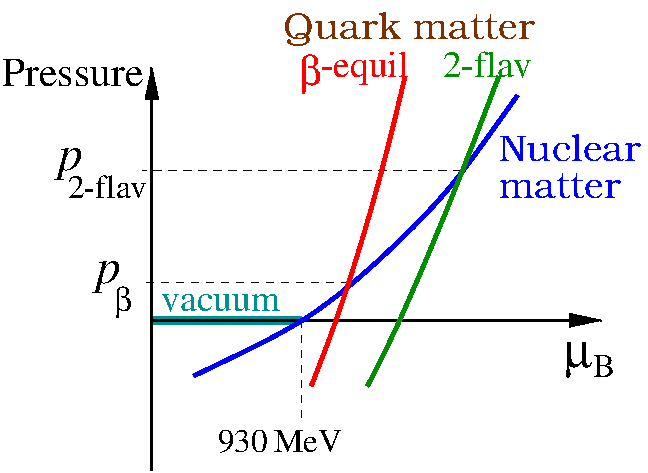
\includegraphics[width=0.65\columnwidth]{Plots/pressure_mu_pos.pdf}%
  \caption{ \mga{Pressure of chemically equilibrated nuclear matter and $uds$ quark matter, and also $ud$ quark matter. We study the regime of pressure
  $P$ between $P_{uds}$ and $P_{ud}$, where $uds$ quark matter is favored over nuclear matter, but
  $ud$ quark matter is not.}
  } \label{fig:pressure-mu}
\end{figure}


\begin{figure}[t]
  \centering
  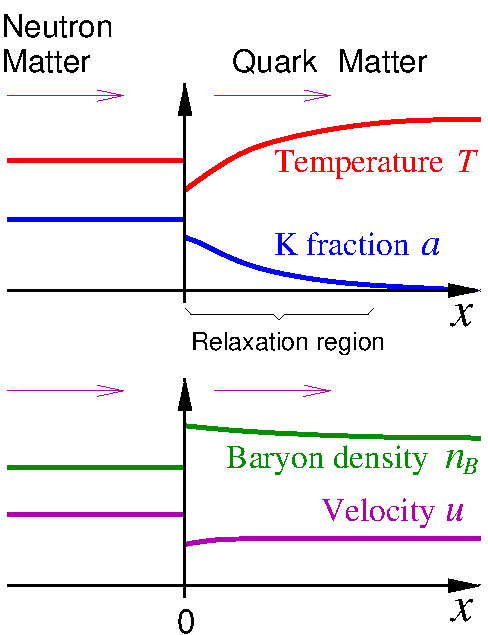
\includegraphics[width=0.65\columnwidth]{Plots/boundary_schematic.pdf}%
  \caption{
  \mgacom{Now that we are doing isothermal and adiabatic cases, we either need different versions of this figure, or drop it.}
  Schematic illustration of the expected boundary profile. Note the discontinuities in some thermodynamic properties at the phase boundary located at $x=0$, followed by relaxation to beta equilibrium as $x\to\infty$.
  } \label{fig:boundary_schematic}
\end{figure}

\section{Formalism and assumptions}
\label{sec:formalism}

\subsection{Main assumptions}

We assume the phase boundary is well approximated as a flat plane which can therefore be modeled as a one-dimensional system. This is a reasonable approximation for neutron star mergers, where the curvature of the boundary is on the kilometer scale, while its thickness is of order micrometers \mga{(see Eq.~\eqref{eq:conversion-thickness})}.
We defer any discussion of instabilities that would lead to a more complicated front geometry.
 \AHcom{As far as I know, people assume that instabilities work on the cm scale, which would still give us many orders of magnitude compared to micrometer. So the planar assumption should be fairly solid}
We assume that the surface tension of the phase boundary is large enough that mixed phases are not favored. We model the nuclear phase as pure neutron matter described by the QMC-RMF3 mean field theory~\cite{Alford:2022bpp,Alford:2023rgp,qmc_rmf3}. We model quark matter as a Fermi gas of massless noninteracting up, down, and strange quarks~\cite{Chodos:1974je,Farhi:1984qu}.

We will follow the standard approach to nuclear to quark conversion \cite{Olinto:1986je,Bombaci:2000cv,Bhattacharyya:2006vy,Niebergal:2010ds,Furusawa:2015vfn,Rosero-Gil:2020caj}
which exploits the clear separation between strong-interaction-driven processes such as local thermal equilibration and deconfinement (which can be treated as instantaneous on the time scales relevant to neutron star mergers) and flavor equilibration, which occurs via weak interactions and is therefore much slower and must be treated explicitly.  We focus on the fastest flavor equilibration channel, the nonleptonic process
\begin{equation}
    d\ u \leftrightarrow u\ s\ .
\label{eq:nonleptonic}
\end{equation}
This equilibrates the quantum number that we will call ``K'', which measures the imbalance between down and strange quarks. 
We ignore electromagnetism, electrons, and neutrinos. We therefore neglect Urca processes, which are generally slower than the non-leptonic process \cite{Alford:2006gy,Alford:2025tbp,Sad:2007afd}, so their inclusion will make the boundary speed even lower.

As noted above, we assume local thermal equilibration is fast enough so that each fluid element has a well-defined temperature $T$. 
\mga{We will first write down the hydrodynamic equations that describe the movement of the fluid, including radiative loss and diffusion of flavor (the $K$ quantum number) and heat.
In the body of the paper, however, we will
not explicitly treat the radiation or diffusion of heat via thermal conduction. Instead, we will calculate the boundary
propagation speed for two extreme cases: adiabatic (no thermal conduction) and isothermal (the whole system is thermally equilibrated to the same temperature).
}

\subsection{Formalism}

To calculate the speed at which the nuclear/quark phase boundary propagates through neutron matter, we will look for a steady state solution to the equations that describe the propagation of a deflagration front. 

We work in the rest frame of the phase boundary, which is located at $x=0$,
as illustrated schematically in Fig.~\ref{fig:boundary_schematic}.
At $x<0$ there is pure neutron matter which we take to be homogeneous, neglecting any disturbance propagating ahead of the phase boundary. The neutron matter flows towards the boundary with a velocity $u(x=0^-)$, which we aim to calculate. Matter at $x=0^-$ immediately (via strong interactions that are instantaneous on the timescales we consider) deconfines into denser quark matter at $x=0^+$ with enough strangeness to be created from neutron matter while conserving energy. (In the example shown in Fig.~\ref{fig:boundary_schematic} this is an endothermic reaction, so the temperature of freshly created quark matter at $x=0^+$ is less than in the neutron matter arriving at $x=0^-$.)  
\AHcom{I don't understand the enough strangeness part?}
\mgacom{If the quark matter doesn't have enough strangeness then it won't be energetically favored (extreme case: udd matter).}

At $x>0$ there is a conversion region where strange quarks are created via the weak interaction, leading to a gradient in the K fraction that drives diffusion of strange quarks 
upstream towards the boundary. This is how the freshly created quark matter at $x=0^+$ can immediately have a larger strangeness fraction than was present in the incoming neutron matter. As $x\to\infty$ the quark matter approaches a fully beta-equilibrated state.

% As noted above, we assume that at each position $x$ the matter is locally thermally (though not chemically) equilibrated with a temperature $T$.
The parameters that describe the state of the matter at any given position $x$ are: 
%
\begin{equation}
\begin{array}{l@{\quad}l}
  n_B  & \text{baryon number density} \\
  n_K \equiv \dfrac{n_d-n_s}{2} & \text{``K'' density} \\
  u & \text{velocity in the $x$ direction} \\[0.5ex]
  T & \text{temperature} 
\end{array}
\label{eq:properties}
\end{equation}
%
From these one can, via the nuclear and quark equations of state (see Appendix~\ref{sec:bag_model}), calculate other properties such as pressure $P$, baryon chemical potential $\mu_B$, energy density, and the K chemical potential 
\begin{equation}
    \mu_K=\mu_d-\mu_s \ ,
\end{equation}
which relaxes towards zero via the weak interaction
\eqref{eq:nonleptonic}.

\JS{We also define the local K fraction}
\begin{equation}
 a(x)\equiv\frac{n_K(x)}{n_B(x)}\ .
 \label{eq:a_definition}
\end{equation}

\subsection{Hydrodynamic equations}
\label{sec:hydro-thermal}


\JS{We work in the phase boundary rest frame and include heat transport while neglecting viscous stresses, so the stress-energy tensor is}
\AHcom{what would a dissipative correction look like as this would also be a result of the same weak interactions I think? du us BV is resonant at very low temperatures}
\begin{equation}
    \begin{aligned}
    T^{\mu\nu}={}&(P+\eps) U^\mu U^\nu+P g^{\mu\nu}\\
    &\JS{{}+U^\mu q_{\rm th}^\nu+q_{\rm th}^\mu U^\nu}\,,
    \end{aligned}
    \label{eq:stress_tensor}
\end{equation}
and baryon current
\begin{equation}
    J_B^\mu=n_B U^\mu \,,
\end{equation}
where $U^\mu = (\gamma,u,0,0)$ is the four-velocity with $u=\gamma v$ and Lorentz factor $\gamma=1/\sqrt{1-v^2}$.
\JS{The heat four current $q_{\rm th}^\mu$ satisfies $U_\mu q_{\rm th}^\mu=0$ and is purely spatial in the local fluid rest frame~\cite{Eckart:1940te}.}
\JS{Baryon number is conserved, while escaping neutrinos can carry energy and momentum out of the fluid:}
\begin{equation}
\begin{aligned}
    \partial_\mu T^{\mu\nu}&=\JS{-\mathcal S^\nu} \, ,\\
    \partial_\mu J_B^\mu&=0 \, .
\end{aligned}
\end{equation}

\mgacom{Is this where we introduce terms corresponding to thermal conduction and radiative energy loss?}

\JS{Here $\mathcal S^\nu$ is the neutrino energy-momentum loss per unit spacetime volume, with $Q_\nu\equiv\mathcal S^0\geq0$ the energy loss per unit volume and time in the phase boundary rest frame.
We impose steady planar flow, so all fields depend only on $x$.
For the slow flows considered here, we model the conductive heat flux by Fourier's law,
\begin{equation}
    q_{\rm th}^x=-\kappa_{\rm th}\frac{dT}{dx}\,,
    \label{eq:fourier_heat_flux}
\end{equation}
where $\kappa_{\rm th}\geq0$ is the thermal conductivity.
The minus sign directs heat toward lower temperature.
This approximation assumes that the heat current relaxes on a time scale short compared with changes experienced by the fluid~\cite{Lander:2018cvq}.
We retain the leading conductive energy flux and neglect the acceleration correction to the relativistic heat law and the heat-current contribution to the momentum flux.
We also neglect neutrino momentum loss, which is suppressed by the fluid speed for isotropic emission in the local rest frame.
In quark matter, $\kappa_{\rm th}$ is determined by quark scattering~\cite{Heiselberg:1993cr}.%; it is a separate transport coefficient from the K diffusion coefficient $D_K$.
}

Weak interactions violate the conservation of the K current,
\begin{equation}
    \partial_\mu J_K^\mu = -\Gamma_K,
\end{equation}\\
%+ \frac{d}{dx}\Big(D \frac{d n_k}{dx}\Big)
%\LBcom{I wanted to write this like baryon and energy-momentum conservation so I think I could be neglecting a time-derivative term?}\\
\hide{
\JScom{I think if we want to write a relativistic 4-vector K current, then we need also to provide it's explicit form just like what we did for $J_B^\mu = n_B U^\mu\ $. Also, $J_K^\mu\neq n_K U^\mu$ because there's K diffusion term in $J_K^x\ $, so we need to be careful. 
In fact,
\[
J^\mu_K = n_K U^\mu + V^\mu\,,\quad \mbox{where}\quad V^\mu = (V^0, -D_Kn_K', 0, 0)
\]
and $V^0$ satisfies $U_\mu V^\mu = 0$ because $J^\mu_K = n_K U^\mu + V^\mu$ is a 1+3 decomposition of $J_K^\mu\ $.
}\\
}
\LBcom{the diffusion term should indeed stay in $J_K^\mu$ because it does not lead to the non conservation of K current unlike the weak interactions.}\\
where $\Gamma_K$ is the rate of down to strange quark conversion (see Appendix~\ref{sec:K-creation}) \LB{and 
\begin{equation}
    J_K^\mu = n_K U^\mu + D_K^\mu,
\end{equation}
where $D_K^\mu$ is the strong-interaction-driven K diffusion current
\begin{equation}
    D_K^\mu = \JS{-}D_K(g^{\mu\nu}\JS{+}U^\mu U^\nu)\partial_\nu n_K.
\end{equation}
See Appendix~\ref{sec:K-diffusion} for our approach to estimating the diffusion coefficient $D_K$. This definition ensures that $U_\mu D_K^\mu=0$, i.e. that there is no time component of diffusion in the local fluid rest frame. 
}
\hide{
\JS{$J_K^\mu$ is the K current, which is given by the following 1+3 decomposition:
\begin{equation}
J^\mu_K = n_K U^\mu + V^\mu\,,\quad \mbox{where}\quad V^\mu = (V^0, -D_Kn_K', 0, 0)\ .
\label{eq:JK_relativistic}
\end{equation}
$U^\mu$ is the relativistic fluid element four velocity, and $V^\mu$ is the spacial component of $J^\mu_K$ in the fluid element co-moving tetrad that carries information of K diffusion. 
}\AHcom{not every current is conserved, the K current in fact should not be conserved but has a source term}
}

The spatial component of the K current $J_K\equiv J_K^1$ is
\LB{
\begin{equation}
    J_K = un_K - \gamma^2 D_K\frac{d}{dx}n_K \ ,
\end{equation}
}
\LBcom{in the relativistic formalism, there is a $\gamma^2$ factor in front of the $D_K$ coefficient so this may need to be propagated forward in the paper.}
where $D_K$ is the strong-interaction-driven K diffusion coefficient, described in Appendix~\ref{sec:K-diffusion}.
\JS{In the transport equations below we use $\gamma^2\simeq1$, appropriate to $u\ll1$, while retaining the relativistic form of the ideal-fluid fluxes.}

\JS{The time component of the energy-momentum balance gives $dT^{x0}/dx=-Q_\nu$.
To leading order in the heat-transport corrections, $T^{x0}$ is the sum of the advective flux $(P+\eps)u\gamma$ and the conductive flux $-\kappa_{\rm th}T'$.
Weak equilibration converts chemical energy into heat within the fluid; this energy is included in the equation of state, so $\Gamma_K$ does not enter as an additional source of total energy.
The steady hydrodynamic equations, with heat transport treated in this slow-flow approximation, are}
\mgacom{add in thermal diffusion and radiation terms}
%
\begin{subequations}\label{eq:front_system_thermal}
\begin{align}
\frac{d}{dx}(u n_B)&= 0\,, 
\label{eq:baryon_conservation_thermal}\\
\frac{d}{dx}\Big((P+\eps) u \gamma - \kappa_{\rm th}\frac{dT}{dx}\Big) &=-Q_\nu\,,
\label{eq:energy_conservation_thermal}\\
 \frac{d}{dx}\big((P+\eps) u^2+P\big)&=0\,,
 \label{eq:momentum_conservation_thermal}\\
 \frac{d}{dx}J_K &= -\Gamma_K\,.
    \label{eq:K_conservation_thermal}
\end{align}
\end{subequations}

\JS{We use two limits of Eq.~\eqref{eq:front_system_thermal} to study the effect of heat transport.
For $\kappa_{\rm th}\to\infty$ and $Q_\nu=0\ $, $dT/dx\to0$ in each phase.
Assuming thermal contact with no temperature jump at the interface gives a single temperature across both phases, the isothermal case of Sec.~\ref{sec:speed-isothermal}.
The conductive flux can remain finite in this limit and balance changes in the advective flux.
For $\kappa_{\rm th}=0$ and $Q_\nu=0$, Eq.~\eqref{eq:energy_conservation_thermal} instead gives $d[(P+\eps)u\gamma]/dx=0$, the adiabatic case of Sec.~\ref{sec:speed}.
Here \emph{adiabatic} excludes conductive and radiative heat loss; weak reactions can still produce entropy.
We set $Q_\nu=0$ in both calculations, consistent with our omission of neutrinos and Urca processes.
}

\section{Boundary propagation speed: isothermal case}
\label{sec:speed-isothermal}

\mgacom{Need to write this}

We now describe how to calculate $u(0^-)$, the speed at which the nuclear/quark phase boundary propagates through neutron matter, in the limit where there is a single uniform temperature across both phases.

\begin{figure}
    \centering
    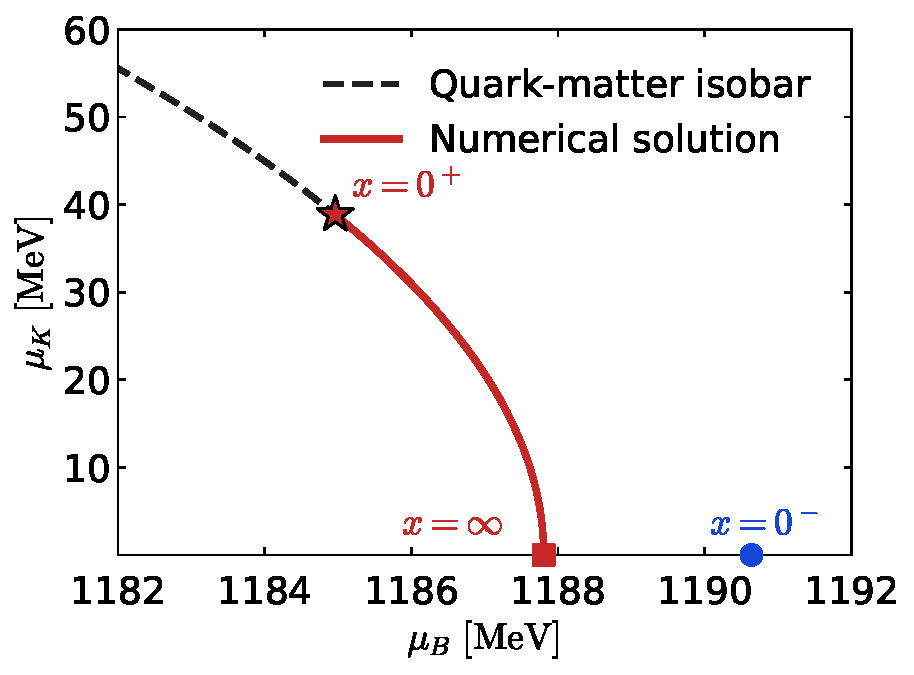
\includegraphics[width=\linewidth]{Plots/isothermal_muB_muK_plane.pdf}
    \caption{Caption}
    \label{fig:isothermal_constant_pressure_trajectory}
\end{figure}

\JS{
This is the $\kappa_{\rm th}\to\infty$ limit described in Sec.~\ref{sec:hydro-thermal}, with finite heat transport maintaining a uniform temperature.\JScom{citations}
\LBcom{Are we sure we cannot impose energy conservation $hu=const$ as well as have constant temperature? I am not sure what the additional unknown quantity would be though.}
The energy balance in Eq.~\eqref{eq:energy_conservation_thermal} still includes conductive transport, so it does not require the advective flux $(P+\eps)u\gamma$ to be constant.
This idealization allows heat exchange with the surroundings to maintain the common temperature.
We solve for the matter profile using $T(x)=T(0^-)$ in place of the energy equation:
%
\begin{subequations}\label{eq:front_system_isothermal}
\begin{align}
\frac{d}{dx}(u n_B)&= 0\,, 
\label{eq:baryon_conservation_isothermal}\\
\frac{d}{dx}T(x) &=0\,,
\label{eq:isothermal_condition}\\
 \frac{d}{dx}((P+\eps) u^2+P)&=0\,,
 \label{eq:momentum_conservation_isothermal}\\
 \frac{d}{dx}J_K &= -\Gamma_K.
    \label{eq:K_conservation_isothermal}
\end{align}
\end{subequations}
%

Most of the piecewise-constant derivation of Sec.~\ref{sec:hydro_analytic} survives this replacement, with one subtlety being that $\mu_B$ and $n_B$ for $x>0$ are no longer constant, but their change is still quite small.  
So figuratively, see Fig.~\ref{fig:isothermal_constant_pressure_trajectory}, when we go from $x=0^+$ to $x = \infty$ in the isothermal limit, instead of moving along the isobar of quark matter on $(T, \mu_K)$ plane for constant $\mu_B\ $, we move along the isobar on $(\mu_B, \mu_K)$ plane for constant $T\ $. 

Along this isobar, $\mu_B$ and $\mu_K$ are not independent.
At fixed $T$, the Gibbs--Duhem relation $dP=n_Bd\mu_B+n_Kd\mu_K$ gives
\begin{equation}
 \left.\dfrac{d\mu_B}{d\mu_K}\right|_{P,T}=-\dfrac{n_K}{n_B}=-a\,,
\label{eq:isobar_gibbs_duhem}
\end{equation}
Therefore, $\mu_B$ increases as weak reactions reduce $\mu_K$, but the change becomes smaller as the matter approaches flavor equilibrium.
For the representative profile with $T=10\,\MeV$, $n_B(0^-)=3n_0$, $B^{1/4}=189.2\,\MeV$, and $a(0^+)=0.146$, $\mu_B$ and $n_B$ increase by only $0.24\%$ between $0^+$ and $x\to\infty$.
Since $a=n_K/n_B$, its exact derivative is $a'=n_K'/n_B-a n_B'/n_B\,.$
Along the same trajectory, the approximation $a'\simeq n_K'/n_B$ differs from the exact derivative by at most $0.47\%$.
We therefore neglect the small variation of $n_B$ in the analytical approximation below.

Baryon and momentum flux conservation are unchanged, so the interface gradient in Eq.~\eqref{eq:interface_gradient}, the integrated K-ness balance in Eq.~\eqref{eq:integrals}, the estimate of $I_1$ in Eq.~\eqref{eq:I1-result}, and the general speed relation in Eq.~\eqref{eq:speed_general} carry over to the isothermal case.
The only remaining change is the evaluation of $I_2$.

As in the piecewise-constant treatment, we fix $\mu_q$ at a representative value.
The coefficients $D_K$, $\gamma_K$, and $\eta$ are then constant, and Eq.~\eqref{eq:I2_definition} reduces to
\begin{equation}
\begin{array}{rl}
 I_2 &= D_K\gamma_K\dsp\int_0^{a(0^+)}\left(a^3+\eta a\right)da \\[2ex]
 &= \dfrac{D_K\gamma_K\,a^2(0^+)\left[a^2(0^+)+2\eta\right]}{4}\,.
\end{array}
\label{eq:I2_isothermal}
\end{equation}
This integral is simpler than its counterpart in Sec.~\ref{sec:hydro_analytic}, where $T(x)$ follows the isobar in Eq.~\eqref{eq:constant_pressure_path}.
In that case, $D_K[T(a)]$ remains inside the integral and produces the $A^{7/3}$ prefactor and the fractional powers in Eq.~\eqref{eq:speed_modified}.

Substituting Eq.~\eqref{eq:I2_isothermal} into Eq.~\eqref{eq:speed_general} gives
\begin{equation}
 u^2(0^-)=\frac{D_K\gamma_K\,a^2(0^+)\left[a^2(0^+)+2\eta\right]}
 {2\lambda_n^2\left[1-a(0^+)\right]\left[1+\xi a(0^+)\right]}\,,
\label{eq:speed_isothermal}
\end{equation}
where $\eta=9\pi^2T^2/\mu_q^2$, and $\lambda_n$ and $\xi$ are defined in Eqs.~\eqref{eq:lambda-def} and \eqref{eq:I1-result}, respectively.
The two terms in brackets arise from the cubic and linear contributions to the weak source in Eq.~\eqref{eq:cubic_rate}.
The cubic contribution dominates when $a(0^+)\gg\sqrt{\eta}$, while the thermal contribution dominates at smaller $a(0^+)\,.$

The parameter $A$ does not appear in the isothermal result because its defining condition, $T(0^+)=0$, belongs to the temperature-varying isobar used in Sec.~\ref{sec:hydro_analytic}.
%Here, the upper limit on $a(0^+)$ must instead be obtained from the static interface condition $P(0^+)=P(0^-)$.
%Moreover, Eq.~\eqref{eq:speed_isothermal} vanishes only as $a(0^+)\to0$ and therefore does not, by itself, determine a zero-speed density.

%To obtain an upper limit on the velocity, since in the isothermal limit, $D_K, \gamma_K, \eta$ and $\lambda_n$ are all constants to very good approximation, the only variable left to tune is $a(0^+)$, and the speed increases with increasing $a(0^+)\ $.
%An obvious upper limit on $a(0^+)$ is $a(0^+)\leq1$, which corresponds to the K fraction in neutron matter, where the velocity blows up. 

Unlike in the energy-conserving case Eq.~\eqref{eq:front_system} and consequently Eq.~\eqref{eq:speed_modified}, where we can maximize the velocity by setting $a(0^+)=A$ where $T(0^+) = 0\ $, in the isothermal limit there's only one obvious upper limit on $a(0^+)$, which is $a(0^+)\leq1$, corresponding to no strangeness in quark matter at $x = 0^+\ $, where the velocity blows up.
Therefore, we cannot maximize the velocity simply by setting $a(0^+)=1\ $. 

We do not know the value of $a(0^+)\ $, but $u(0^-)$ is a monotonically increasing function of $a(0^+)$ in the domain $0<a(0^+)<a(0^-)=1$ for $\xi = 0\ $, so to obtain an upper bound on the isothermal boundary speed $u_\text{max}(0^-)$ we need to find the $a_\text{max}(0^+)$ in the isothermal limit, which we denote by $A'$, and it's the value of $a(0^+)$ at which the quarks at the boundary have the same average chemical potential $\mu_B(0^+) + n_K(0^+)\mu_K(0^+)/n_B(0^+)$ as the quarks in the baryons. 
Quark matter with $a(0^+)>A'$ would have insufficient strangeness to make it favored over neutron matter \cite{Alford:2014jha}. 

%In our plots we calculate $a_{\text{max}}(0^+)$ numerically, but
Taylor-expanding the quark matter EoS around its beta-equilibrated state, we can obtain an approximate formula that in the parameter range that we explored agrees with the numerical result to within 1\%,
\begin{equation}
A' \approx \sqrt{ \dfrac{2 \bigl(\mu_B(0^-) - \mu_B(\infty)\bigr)}{n_B(\infty)}\left. \dfrac{\partial^2 P_\text{QM}}{\partial\mu_K^2}\right|_{\infty}} \ .
\label{eq:a0plus_max}
\end{equation}

Since Eq.~\eqref{eq:speed_isothermal} has monotonic dependence on $a(0^+)$, and we know that $0<a(0^+) < A'<1$, similar to Eq.~\eqref{eq:speed_scaling}, we can do the same thing for Eq.~\eqref{eq:speed_isothermal}
\begin{equation}
\begin{aligned}
u_{\max}(0^-)\simeq&(98\, {\rm m/s})
\frac{n_B(\infty)}{n_B(0^-)}\\
&\times\left(\frac{\mu_B(0^+)}{1200\ {\rm MeV}}\right)^\frac{17}{6}
\left(\frac{10\ {\rm MeV}}{T}\right)^\frac{5}{6}\\
&\times\frac{A'\sqrt{(A')^2+162\pi^2T^2/\mu_B^2(0^+)}}
{\alpha_s^{5/6}\sqrt{1-A'}\sqrt{1+\xi A'}}\ .
\end{aligned}
\label{eq:isothermal_speed_scaling}
\end{equation}
}

\section{Boundary propagation speed: adiabatic case}
\label{sec:speed}


\subsection{Adiabatic hydrodynamic equations}
\label{sec:hydro-equations}

\JS{Setting $\kappa_{\rm th}=0$ and $Q_\nu=0$ in Eq.~\eqref{eq:front_system_thermal} gives the adiabatic steady-front equations}
%
\begin{subequations}\label{eq:front_system}
\begin{align}
\frac{d}{dx}(u n_B)&= 0\,, 
\label{eq:baryon_conservation}\\
\frac{d}{dx}((P+\eps) u \gamma) &=0\,,
\label{eq:energy_conservation}\\
 \frac{d}{dx}((P+\eps) u^2+P)&=0\,,
 \label{eq:momentum_conservation}\\
 \frac{d}{dx}J_K &= -\Gamma_K.
    \label{eq:K_conservation}
\end{align}
\end{subequations}
%

%\AHcom{mix of j and J?}
% and $D$ is the strong-interaction-driven K diffusion coefficient, described in Appendix~\ref{sec:K-diffusion}

Eqs.~\eqref{eq:baryon_conservation}, \eqref{eq:energy_conservation}, \eqref{eq:momentum_conservation}
are flux conservation laws, stating that the baryon, momentum, and energy fluxes
\begin{equation}
\left.
\begin{array}{rl}
 J_B &=n_Bu \,, \\[1ex]
 \Pi &=hu^2+P \,, \\[1ex]
 E &=hu\sqrt{1+u^2}\,.
\end{array}
\right\}\parbox{6em}{Independent of $x$}
\label{eq:conserved_fluxes}
\end{equation}
have fixed values at all $x$, while other thermodynamic and compositional properties will vary through the boundary and relaxation region.

To obtain the profile of the moving phase boundary we only need to solve the remaining Eq.~\eqref{eq:K_conservation}, a second-order differential equation that can be recast as two first-order differential equations for the K density and current
\begin{subequations}
\label{eq:reduced_BVP}
\begin{align}
 \frac{d}{dx}n_K &=\frac{un_K-J_K}{D_K}\,,\JS{\quad x>0\,,}
\label{eq:BVP_nK}\\
 \frac{d}{dx}J_K &=-\Gamma_K\,.
\label{eq:BVP_jK}
\end{align}
\end{subequations}
\JS{However, it's worth noting that diffusion of quarks and hence K-ness is only possible in deconfined quark matter at $x>0\ $, so Eq.~\eqref{eq:BVP_nK} is only defined for $x>0\ $. For $x<0\ $, we have $dn_K/dx = 0$ and $J_K = un_K\ $.}
\mgacom{Our assumption that the nuclear matter is all neutrons makes K diffusion nonexistent there.}
There is now a well defined procedure for constructing a solution to these differential equations. 
Assume we have solved them up to some position $x$, giving $n_K(x)$ and $J_K(x)$. We can combine this with the already-specified values of the conserved fluxes \eqref{eq:conserved_fluxes} and the quark matter equation of state (Appendix~\ref{sec:bag_model}) to solve for the remaining properties of the matter at $x$, such as $n_B(x)$, $u(x)$, $\mu_B(x)$, $\mu_K(x)$, \mga{$T(x)$}, etc. This allows us to calculate $D_K(x)$ and $\Gamma_K(x)$ (see Appendices~\ref{sec:K-creation} and \ref{sec:K-diffusion}) and thereby obtain $n_K(x+\de x)$ and $J_K(x+\de x)$.


\subsection{Boundary conditions}

To construct the boundary profile we need 5 initial conditions  specifying the state of the incoming nuclear matter: $n_B(0^-)$, $n_K(0^-)$, $dn_K/dx(0^-)$, $T(0^-)$, $u(0^-)$. However, since we assumed the incoming matter is  neutron matter, for which $n_K=n_d/2$, we have
\begin{equation}
  n_K(0^-)=n_B(0^-)\,,
  \label{eq:nK-nuclear}
\end{equation}
and since we have assumed the neutron matter is homogeneous,
\begin{equation}
  \dfrac{dn_K}{dx}(0^-)=0\,,
  \label{eq:dnKdx-nuclear}
\end{equation}
so we only need to specify $n_B(0^-)$,  $T(0^-)$, $u(0^-)$, which fixes the conserved fluxes $J_B$, $\Pi$, and $E$ for the whole solution.  

Since the solution must yield equilibrated quark matter as $x\to\infty$, we also impose the boundary condition $\mu_K(\infty)=0$, which for our model of quark matter is equivalent to $n_K(\infty)=0$. This turns \eqref{eq:reduced_BVP} into an eigenvalue problem, where for given 
$n_B(0^-)$ and $T(0^-)$ there is only one value of the incoming neutron matter velocity $u(0^-)$ that yields a valid solution.
This will yield our desired result, the speed at which the boundary propagates through neutron matter, as a function of the density and temperature of the neutron matter.

The first step in solving the equations is to relate the K density and current at $x=0^+$ to the initial conditions at $x=0^-$, after which we can evolve the solution to $x=+\infty$ using \eqref{eq:front_system}.

\JS{%Only one of the two equations in \eqref{eq:reduced_BVP} is a genuine conservation law. Eq.~\eqref{eq:BVP_jK}, $dJ_K/dx=-\Gamma_K$, has $J_K$ as its conserved current, so integrating it across the interface leaves $J_K$ continuous, since the source term contributes nothing as the interface width goes to zero. Eq.~\eqref{eq:BVP_nK} is not a conservation law for $n_K$: it is a constitutive relation, defining $J_K$ in terms of $n_K$ and its gradient
\mgacom{I don't think this is an essential difference. It's still an equation of the form $dF/dx = RHS$. In order for there to be a discontinuity in $F$ there must be a delta-function in $RHS$. I think the essential point is that we know the RHS of \eqref{eq:BVP_jK} doesn't have a delta fn, but we can't rule it out for the RHS of \eqref{eq:BVP_nK}}
\JScom{I think the problem is $D_K$ in Eq.~\eqref{eq:BVP_nK} is not even defined for $x\leq 0$, so I don't think we can claim $n_K(0^-)\neq n_K(0^+)$ implies $J_K$ have delta fn part. The only meaningful equation that can be integrated across $x=0$ is Eq.~\eqref{eq:BVP_jK}, and we need to make it clear that Eq.~\eqref{eq:BVP_nK} is only defined for $x>0\ $, and that $J_K = n_K u$ for $x<0$ and $J_K = n_K u - D_K n_K'$ for $x>0\ $.}
\mgacom{You are focusing on the right side of (13a), saying it only takes that form in quark matter. That's true, but it avoids the key question, which is whether the true right side of (13a) could have a delta function at $x=0$. If there is a discontinuity in $n_K$ then the true RHS of (13a) must have such a delta function.}
%through the quark-matter diffusion coefficient $D_K$, which has no counterpart on the nuclear side. Nothing therefore forces $n_K$ to be continuous across the interface, consistent with deconfinement reprocessing the composition of the newly formed quark matter instantaneously.
}

Integrating Eqs.~\eqref{eq:reduced_BVP} across the sharp interface yields the hydrodynamic jump condition
\begin{equation}
 u(0^+)n_K(0^+)
 -\left[D_K\frac{dn_K}{dx}\right]_{0^+}
 =u(0^-)n_K(0^-)\,.
\label{eq:jump_K-}
\end{equation}
We do not need to know the K diffusion coefficient on the nuclear side because we have assumed there is no gradient there. Eq.~\eqref{eq:jump_K-} fixes $dn_K/dx(0^+)$ in terms of $n_K(0^+)$ but we have no constraint on $n_K(0^+)$ so we have to treat it 
%(or equivalently $a(0^+)$) 
as an additional parameter of the system. In our calculations we will choose the value of $n_K(0^+)$ that maximizes the speed of the boundary.

We can now obtain the boundary speed in terms of the density and temperature of the neutron matter and the K fraction in the freshly created quark matter. We do this by solving \eqref{eq:reduced_BVP} as described in Sec.~\ref{sec:hydro-equations} using the boundary conditions described above.

One approach is to solve the differential equations numerically, as described in  Appendix~\ref{sec:numerical}, and this is how most of our results in Sec.~\ref{sec:results} were obtained. However, as we now describe, one can also formulate an approximate analytic solution, which is helpful for interpreting the results. 



\subsection{Piecewise-constant analytical approximation}
\label{sec:hydro_analytic}

\mgacom{Could we think of a more informative name for this approximation? E.g. "constant pressure" or similar.}

If the boundary propagation speed is much less than the speed of light, then, as we see in our full numerical calculations (see Fig.~\ref{fig:numerical}) the boundary profile exhibits noticeable simplifying features. One can treat $n_B\,,$ $u\,,$ $\mu_B\,,$ $P\,,$ and
$h$ as independent of $x$ on the quark matter side, while retaining the $x$ dependence of temperature $T(x)\,,$ and K density $n_K(x)\ $.%(and hence $\mu_K(x)$ and $a(x)$).
%\LBcom{This is the first time we mention $a(x)$ so it is not obvious what this means.}\JScom{We could just move this somewhere after Eq.~\eqref{eq:a_definition}.}
As we will now show, this allows us to find an analytic expression for the speed of the boundary.

We write the $x$-independent baryon density in the quark matter as
\begin{equation}
n_B^{(+)} \equiv n_B(x) \quad \forall x>0 \,,
\label{eq:nBplus-def}
\end{equation}
\mgacom{I am open to alternative notations for the constant quantities}
and define $\Bratio$ (which will always be less than 1) as the ratio of neutron matter to quark matter baryon density at the transition,
\begin{equation}
    \Bratio \equiv \dfrac{n_B(0^-)}{n_B^{(+)}} \,,
    \label{eq:lambda-def}
\end{equation}
so the $x$-independent velocity of the quark matter is
\begin{equation}
u^{(+)} =\Bratio u(0^-)\,.
\label{eq:uplus-def}
\end{equation}
\JS{Since $n_B$ is independent of $x$, it is natural to work in terms of the local K fraction $a(x)$ defined in Eq.~\eqref{eq:a_definition}.}

To find the speed $u(0^-)$ we use Eq.~\eqref{eq:jump_K-}
along with
\eqref{eq:nBplus-def}, \eqref{eq:lambda-def}, \eqref{eq:uplus-def} to obtain
\begin{equation}
% \dfrac{D_K(0^+)}{n_B(0^-)}\dfrac{d n_K}{dx}\biggr|_{0^+}
%\biggl( \dfrac{n_K(0^+)}{n_B(0^+)} - \dfrac{n_K(0^-)}{n_B(0^-)} \biggr)^{\!-1}
\begin{array}{rl}
u(0^-)  &= -\dfrac{D_K(0^+)a'(0^+)}{\Bratio \bigl(1-a(0^+)\bigr)}  \,,\\[3ex]
a'(x) &\equiv \dfrac{da}{dx} = \dfrac{1}{n_B^{(+)}} \dfrac{dn_K}{dx} \,.
 \end{array}
\label{eq:interface_gradient}
\end{equation}
The boundary conditions determine $\Bratio$ and $a(0^+)$, but
$D_K(0^+)a'(0^+)$ is determined by the requirement 
that $a(\infty)=0$. To impose this exactly we would have to evolve $a(x)$  from $x=0^+$ to infinity using the K current equation Eq.~\eqref{eq:reduced_BVP}.

We cannot solve this equation exactly in full generality, but we can make a good estimate of the result. Multiplying Eq.~\eqref{eq:BVP_jK} by $D_K(x)a'(x)$, using Eq.~\eqref{eq:BVP_nK} to eliminate $J_K$, and integrating from $x=0^+$ to infinity, we find 
\hide{
\begin{equation}
\begin{array}{rl}
 \dfrac{1}{2} \Bigl( D_K(0^+)\,n_K'(0^+)\Bigr)^{\!2}
 = &-\,u^{(+)}\!\!\dsp\int_{0^+}^\infty \!\!\!  D_K(x)\,\bigl(n_K'(x)\bigr)^2 \, dx\\[2ex] 
  -&\dsp\int_{0^+}^\infty \!\!\! D_K(x)\,n_K'(x) \Gamma_K(x) \, dx
\end{array}
\end{equation}
}
\begin{equation}
 \dfrac{1}{2} \Bigl( D_K(0^+)\,a'(0^+)\Bigr)^{\!2} = -u^{(+)}I_1 + I_2 \,,
 \label{eq:integrals}
\end{equation}
where $I_1$ and $I_2$ are positive dimensionless integrals over $x$ which can be rewritten as
integrals over $a$, since $a(x)$ is expected to be a monotonically decreasing function over $0^+\leqslant x < \infty$ as the quark matter equilibrates in the conversion region behind the boundary.
\begin{equation}
\begin{array}{rl}
I_1 &= \dsp \int_{0^+}^\infty D_K(x) \bigl(a'(x)\bigr)^2\,dx \,, \\[2ex]
  &= -\dsp\int_0^{a(0^+)} D_K a'\,da \,.
  \end{array}
  \label{eq:I1_definition}
\end{equation}
%
\begin{equation}
\begin{array}{rl}
I_2 &=-\dfrac{1}{n_B^{(+)}}\dsp\int_{0^+}^\infty  D_K \Ga_K a'\,dx \,, \\[2ex]
&= \dfrac{1}{n_B^{(+)}}\dsp\int_0^{a(0^+)} D_K \Ga_K\,da \,.
 \end{array}
\label{eq:I2_definition}
\end{equation}
In an exact calculation both integrands should be obtained from the solution to 
Eq.~\eqref{eq:reduced_BVP}, but we will now show how one can obtain reasonable approximations to both integrals without knowing the solution.


We first estimate $I_1$ because the estimate will turn out to depend on our desired result $u(0^-)$, requiring regrouping of Eq.~\ref{eq:interface_gradient}. We assume that, as we see in the numerical solutions, the
actual profile has $D_K(x) a'(x)$ increasing monotonically from its value $-\Bratio u(0^-)[1-a(0^+)]$ at $x=0^+$ (from Eq.~\eqref{eq:interface_gradient}) to zero at $x=\infty$. This is expected because $a(x)$ decreases monotonically to zero, and any variation in the diffusion constant $D_K$, which depends mainly on the temperature, is too weak to overcome that. We can then parameterize the integral in terms of a ``sharpness'' factor $\xi$:
\begin{equation}
\begin{array}{rl}
 I_1 &= -\dfrac{1+\xi}{2}\,D_K(0^+) a'(0^+)\, a(0^+) \\[2ex]
  &= \dfrac{1+\xi}{2}\,
 \Bratio u(0^-)\,[1-a(0^+)]\,a(0^+)\,.
 \end{array}
 \label{eq:I1-result}
\end{equation}
Here $-1<\xi<1$ characterizes the shape of the diffusion profile. \JS{For details of this sharpness factor $\xi$ and derivation of Eq.~\eqref{eq:I1-result}, see Appendix~\ref{sec:xi-shape}.}
%\mgacom{Explain this in an appendix?}\JScom{Added Appendix~\ref{sec:xi-shape}.}
Substituting this relation into \eqref{eq:integrals} and \eqref{eq:interface_gradient} yields
\begin{align}
 u^2(0^-)&= \frac{2 I_2}
 {\Bratio^2[1-a(0^+)][1+\xi a(0^+)]}\,,
\label{eq:speed_general}
\end{align}


The final step is to evaluate $I_2$, for which we need to know how the K diffusion coefficient $D_K$ and K creation rate $\Gamma_K$ vary though the conversion region. In the piecewise constant approximation the pressure and baryon chemical potential have constant values $P^{(+)}\approx\Pi$ and $\mu_B^{(+)}$ in that region, so the system follows an isobar in the $\mu_K$-$T$ plane.  Moreover, 
since $\mu_K/\mu_B^{(+)}$ is typically of order 0.1 and $T/\mu_B^{(+)}$ is of order 0.03, we can expand the quark matter EoS to quadratic order \eqref{eq:QM-EoS-2nd-order}, so
the isobar takes the form of a quadrant of an ellipse in the $\mu_K$-$T$ plane.
%defined by }
%\begin{equation}
% T(x)^2= T(\infty)^2 - \frac{\mu_K(x)^2}{2\pi^2}\,.\label{eq:ellipse}
%\end{equation}
%
To this order there is a linear relationship between the strangeness fraction $a$ and $\mu_K$ (Eq.~\eqref{eq:a-muK}) so the quark matter follows an elliptical quadrant in the $a$-$T$ plane, as shown in
Fig.~\ref{fig:constant_pressure_trajectory}.


\begin{figure}[t]
  \centering
  \IfFileExists{Plots/T_a_constant_pressure.pdf}{%
    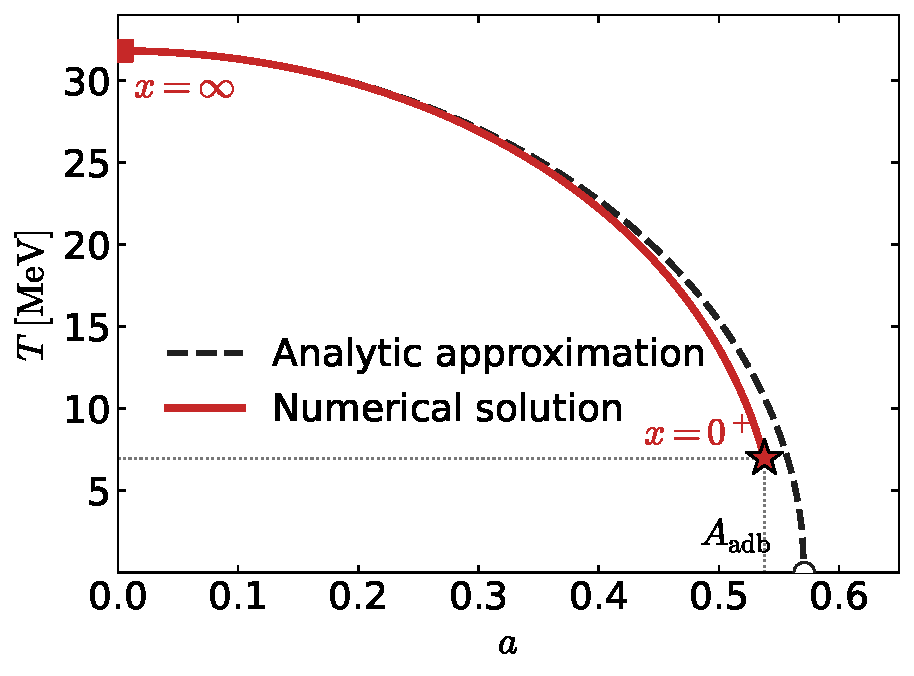
\includegraphics[width=\columnwidth]{Plots/T_a_constant_pressure.pdf}%
  }{%
    \includegraphics[width=\columnwidth]{Hydrodynamical combustion/Plots/T_a_constant_pressure.pdf}%
  }
  \caption{Constant-pressure trajectory through the quark conversion layer.
  The red curve is the energy-conserving numerical profile for
  $T(0^-)=10~{\rm MeV}\,,$ $B^{1/4}=180~{\rm MeV}\,,$
  $n_B(0^-)=3n_0\,,$ and $a(0^+)=0.55$; the dashed curve is the
  quarter ellipse in Eq.~\eqref{eq:constant_pressure_path}.
  The profile runs from the just-deconfined state at $x=0^+$ to the
  equilibrated state at $x\to\infty\,.$  The point $(A,0)$ is the zero-temperature
  endpoint of the extrapolated isobar and need not coincide with the state at $x=0^+\,.$}
\label{fig:constant_pressure_trajectory}
\end{figure}

Using Fig.~\ref{fig:constant_pressure_trajectory} we can describe the conversion region as follows. At $x=0$ the quark matter has some initial K fraction $a(0^+)$ which determines the initial temperature $T(0^+)$ (the red star in the figure ). As $x$ increases, the system moves upwards along the elliptical isobar, ending at $a=0$ and some final temperature when $x\to\infty$ (the red square in the figure).


This gives us a natural way to set a limit on the previously unconstrained parameter $n_K(0^+)$, or equivalently $a(0^+)$. For given initial conditions ($n_B(0^-)$,  $T(0^-)$, $u(0^-)$), the largest possible value for $a(0^+)$ is the one that would give the lowest allowed  initial quark matter temperature, $T(0^+)=0$. Thus, $a(0^+)$ cannot be larger than $A$ \mgacom{I would like to have a more obvious symbol for this, but not sure what would be better}, the
value where the isobar meets the $T=0$ axis
in Fig.~\ref{fig:constant_pressure_trajectory}, defined by
$P_{\text{QM}}(A,T=0)=P^{(+)}$, so \JS{to leading order,}
\begin{equation}
\begin{array}{rl}
a(0^+) &\leqslant A \\[2ex]
A &\JS{\approx}\; \dfrac{3}{2}\dfrac{\sqrt{108\pi^2\bigl( P^{(+)}+ U_{\text{bag}} \bigr) - \bigl(\mu_B^{(+)}\bigr)^4}}{\bigl(\mu_B^{(+)}\bigr)^2}
\end{array}
\label{eq:a-max}
\end{equation}
%\mgacom{I'm not sure how useful this is (do we have a simple way to determine $\mu_B^{(+)}$? but I want to have an equation for $A$ that we can refer to in the future.}\JScom{In the code using analytical approximation Eq.~\eqref{eq:speed_modified} to get $u(0^-)\ $, I used a leading order analytical expression $A = 9\pi T^{(+)}/(\sqrt{2}\mu_B^{(+)})\ $. To get $\mu_B^{(+)}\ $, the code uses a ``closure'' method. First guess a $u(0^-)\ $, then use the hydrodynamical jump conditions to solve for $T(0^+)$ and $\mu_B(0^+)$, which is used to calculate $A$ and $u(0^-)$ again, and the code use root finder to make the guessed $u(0^-)$ close in on the calculated $u(0^-)\ $. }

To understand the physics behind this limit, note that larger values of $a(0^+)$ correspond to smaller strangeness fraction in the quark matter that is first created immediately behind the phase boundary,

The isobar in Fig.~\ref{fig:constant_pressure_trajectory} defines the quark matter temperature $T(x)$ as a function of $a(x)$; solving $P_\text{QM}(a,T)=P_\text{QM}(A,0)$ we find 
% Using Eq.~\eqref{eq:ellipse} $A^2=9\pi^2T^2(\infty)/(2\mu_q^2)\ $, and
\begin{equation}
 T^2=\frac{2(\mu_B^{(+)})^2}{81\pi^2}(A^2-a^2)\,
% \eta(a)=2(A^2-a^2)\,,
\label{eq:constant_pressure_path}
\end{equation}
% where the second relation follows from $\eta=9\pi^2T^2/\mu_q^2\,.$   Since $\mu_K$ is proportional to $a$ at this order, Eq.~\eqref{eq:constant_pressure_path} is the same quarter ellipse in either the $(\mu_K,T)$ or $(a,T)$ plane.


We can now evaluate the integral $I_2$ \eqref{eq:I2_definition} by using the results from
Appendices~\ref{sec:K-creation} and \ref{sec:K-diffusion})
for $\Ga_K(a,T)$ and $D_K(a,T)$ (keeping only the first term), and using \eqref{eq:constant_pressure_path} to express $T$ as a function of $a$. We find
\begin{align}
 I_2 = &\dfrac{27 \pi^{7/3}}{56\sqrt{2}}
 \dfrac{A^{7/3}\ga_K}{\al_s^{5/3} h_D \mu_B^{(+)}}\ \times\notag \\
 &\biggl[ 8 + \Bigl(1-\dfrac{a(0^+)^2}{A^2}\Bigr)^{\!1/6}\,\Bigl(\dfrac{a(0^+)^2}{A^2} - 8\Bigr) \biggr] \,.
\end{align}

%
So from \eqref{eq:speed_general},
\begin{align}
 u^2&(0^-)
 =
 \frac{9\pi^{7/3}}
 {4\sqrt{2}\,h_D\alpha_s^{5/3}}\,
 \frac{\gamma_K A^{7/3}}
 {\mu_B^{(+)} \Bratio^2
 \bigl(1-a(0^+)\bigr)\bigl(1+\xi a(0^+)\bigr)}
\notag\\
 &\times
 \left[
 \frac{24}{7}
 -3\left[1-\frac{a^2(0^+)}{A^2}\right]^{1/6}
 -\frac{3}{7}
 \left[1-\frac{a^2(0^+)}{A^2}\right]^{7/6}
 \right]\,.
\label{eq:speed_modified}
\end{align}
We want to find out the fastest speed at which the phase boundary could move, $u_{\text{max}}$, so we will set \azp, the K fraction in freshly created quark matter, to the value that maximizes the speed.
We see from \eqref{eq:speed_modified} that
the speed of the boundary grows as \azp\ gets larger. This follows because
the factor in square brackets has a weak dependence on $a(0^+)$, so the speed is determined by the denominator $\bigl(1-a(0^+)\bigr)\bigl(1+\xi a(0^+)\bigr)$. \old{For any reasonably smooth profile we expect $|\xi|\ll 1$} \JS{After seeing the numerical profile for various $T(0^-)$ and $n_B(0^-)$ we find out $\xi=-0.5$ is a good approximation }(Appendix~\ref{sec:xi-shape}),  but for any value of $\xi$ in its allowed range $(-1,1)$ the denominator shrinks (so the speed grows) as \azp\ grows from 0 towards 1.

This means that to achieve the maximum phase boundary speed for given initial conditions,
%nuclear matter temperature and metastability, 
we need larger \azp, which makes sense because that corresponds to a lower strangeness fraction in the freshly created quark matter, closer to the flavor content of the neutron matter.
As noted above, the largest possible value of \azp\ is $A$, so setting $\azp=A$ we find the maximum speed
\begin{align}
u_{\rm max}(0^-) = (82\,\m\s^{-1})\,
&\dfrac{n_B^{(+)}}{n_B(0^-)}
\biggl(\!\dfrac{\mu_B^{(+)}}{1200\,\MeV}\!\biggr)^{\!2}
\times \notag\\
& \dfrac{ A^{7/6}}{\al_s^{5/6} \sqrt{1-A}\sqrt{1+\xi A}} \, .\label{eq:speed_scaling}
\end{align}
\mga{Thus the typical speed of the boundary is expected to be of order $100\m\,\s^{-1}$.} In this expression the only factor that could drive the speed to a significantly higher value is $1/\sqrt{1-A}$. \mga{To see when $A$ could approach 1} we recall that $A$ is the largest possible K fraction in the freshly created quark matter at $x=0^+$. The K fraction in neutron matter is 1, so \mga{if $A=1$ then we have such a high pressure that} nuclear matter can convert to quark matter with the same flavor content while conserving energy. In this case no weak interactions are needed, so it is not surprising that our approach breaks down.

We can also use the piecewise constant approximation to estimate the thickness $L_{\text{conv}}$ of the conversion region, which determines the range of curvature that is compatible with our assumption of a  planar geometry. If the boundary moves slowly then when $a \ll 9\pi T/\mu_B^{(+)}$, which is guaranteed to occur at large $x$ where $a\to 0$, the K current equation reduces to
\begin{equation}
    \dfrac{d^2 a}{dx^2} =
    \dfrac{\ga_K}{D_K}\biggl(\dfrac{9\pi T}{\mu_B^{(+)}}\biggr)^{\!2} a \,.
\end{equation}
At large $x$ the temperature reaches an asymptotic value $T(\infty)$, so we can estimate the thickness of the conversion region as
\begin{align}
    L_{\text{conv}} &\approx \dfrac{\mu_B^{(+)}}{9\pi T(\infty)}\sqrt{\dfrac{D_K}{\ga_K}} \notag\\
    &= (0.2\,\mu\m)\,\dfrac{1}{\al_s^{5/6}}
    \biggl(\dfrac{1200\,\MeV}{\mu_B^{(+)}}\biggr)^{\!7/6}
     \biggl(\dfrac{10\,\MeV}{T(\infty)}\biggr)^{\!11/6}
    \,, \label{eq:conversion-thickness}
\end{align}
where we evaluated $D_K$ using \eqref{eq:diffusion_coefficient} with $T=T(\infty)$.
and $\gamma_K$ from Eq.~\eqref{eq:cubic_rate}.
This supports our use of the planar approximation, since the typical curvature of a quark/nuclear boundary in neutron stars will be of order kilometers, much larger than the thickness of the boundary.

\mgacom{Edited up to here}

\JS{

\subsection{Thermal conductivity}

Currently we are setting $T(0^+) = 0$ exactly to maximize velocity. Although this can be done in the analytical or semi-analytical approach, numerically I kept running into difficulties. I think now I have a better understanding: $T(0^+) = 0$ leads to $D_K(0^+)\to \infty$ and $D_K^{-1}(0^+) = 0$, which according to Eq.~\eqref{eq:reduced_BVP}, leads to $n_K'(0^+) = 0$. Although there's no infinities and everything seems fine, zero initial condition in derivatives is what people call non-Lipschitz initial condition. 

Why this is problematic? To break it down, this is what the numerical solver sees for $T(0^+) = 0\ $:
\[
\begin{aligned}
& \dfrac{dn_K}{dx}(0) \equiv \frac{n_K(\delta) - n_K(0)}{\delta} = \frac{u n_K - j_K}{D_K}(0) = 0\\
& \dfrac{d j_K}{dx}(0)\equiv \frac{j_K(\delta) - j_K(0)}{\delta} = -\Gamma_K(0)\neq 0
\end{aligned}
\]
after some rearrangements, we get
\[
n_K(\delta) = n_K(0)\,,\quad j_K(\delta) = j_K(0) - \Gamma_K\cdot \delta
\]
So $n_K(\delta) = n_K(0)\ $, which is sensitive to the step size $\delta\ $. This means the solver can return two solutions that numerically solves the equations, but they look different: their $n_K$ profile have different plateau length in the beginning. These two solutions can have $u(0^-)$ and $j_B$ differ by 20\% . 

So to resolve this, I have several plans:
\begin{itemize}
    \item cheapest: when numerically solving the set of equations, don't put in exactly zero $T(0^+)\ $; instead choose a sufficiently small quark matter initial temperature, say $T(0^+) = 0.01$ MeV and spend a sentence or two maybe at the $z(t)$ part explaining thermal conductivity is an interesting future research direction.
    \mgacom{Yes I prefer this approach. You need to make $T(0^+)$ small enough so that the speed no longer depends on it noticeably. Maybe that already happens for values above $0.01\,\MeV$.}
    \item minimal thermal conductivity, where we don't add another full ODE to solve, but just model the thermal conductivity ODE, and just integrate it across $x=0$ to place a lower bound on $T(0^+)\ $
    \item full thermal conductivity modeling. To do this we need to replace the current energy conservation equation $d(h\gamma u)/dx = 0$ by a second order ODE similar to what we have for $n_K\ $ right now:
\[
\frac{d}{dx}\Big(h\gamma u - \kappa_{\rm th}\frac{dT}{dx}\Big) = -Q_\nu
\]
where Eq. (62) in \cite{Heiselberg:1993cr} gives a very similar expression for $\kappa_{\rm th}$ compared with $D_K\ $, and $Q_\nu$ is the energy taken away by neutrinos per unit time. So judging by the similarity, I assume every method: analytical, numerical, whatever we have developed for solving the $n_K$ ODE would also apply here. But the draw back of the full thermal conductivity modeling is that we are not including Urca, so this $Q_\nu$ is essentially zero in our model. We need to explain that away. 
\end{itemize}

}


%For $\alpha_s=0.3\,,$ $\mu_q=300$--$400~{\rm MeV}\,,$ $T=1$--$50~{\rm MeV}\,,$ and order-unity composition, $\tau_{\rm weak}$ is of order nanoseconds and $L_{\rm weak}$ ranges from tens of nano-meters to a few micrometers.  By contrast, a representative stellar gradient $\lvert dn_B/dz\rvert\sim0.3n_0\,{\rm km}^{-1}$ at $n_B\sim3n_0$ corresponds to a density scale height of about $10~{\rm km}\,.$  

%\JScom{This paragraph is trying to further justify piecewise constant for $n_B$ and $P\ $.}
%The expected fractional change in $n_B$ across the conversion layer is therefore at most of order $10^{-10}\,,$ and similar argument applies to the pressure profile as well.  Momentum conservation gives the same conclusion locally: the departure from constant pressure is of relative order $hu^2/P\,,$ while the weak-diffusive estimate $u\sim[D_K\gamma_K]^{1/2}$ is sub-kilometer per second and hence $u^2\lesssim10^{-11}$ in natural units. This scale separation justifies treating the hydrodynamic backgrounds as piecewise constant while retaining the composition and temperature profiles.


%This expression Eq.~\eqref{eq:speed_modified} retains the physical case $a(0^+)<A$; setting $a(0^+)=A$ gives the zero-temperature endpoint.  
%Besides the piecewise-constant hydrodynamic background, the approximations are the quadratic equation-of-state expansion, omission of the subleading $T^2$ term in $D_K^{-1}\,,$ and the profile parameter $\xi\,.$ 


\section{Results}
\label{sec:results}

\begin{itemize}
  \item first, the set up
\end{itemize}

We discuss the energy conserving front system Eq.~\eqref{eq:front_system} first. We choose the bag constant by requiring cold neutron matter and cold equilibrated strange quark matter to coexist at neutron matter critical baryon number density $n_B^{\rm crit}(T{=}0)=3n_0\,.$
This gives $U_{\rm bag}^{1/4}=189.2\,\MeV\,.$
Since we are not including Urca processes, we set strange quark mass to zero.
We also adopt the conventional phenomenological choice $\alpha_s=0.3$ for bag-model quark matter \JS{\cite{Farhi:1984qu,Madsen:1998uh}}. %\JScom{Also talk about and justify the choice of $T(0^+) = 5$ MeV choice.} %, and a fixed interface temperature $T(0^+)=5\,\MeV\,.$
For each pair of upstream variables $n_B(0^-)$ and $T(0^-)\,,$ we evolve the K density and current, reconstruct the local fraction $a(x)=n_K(x)/n_B(x)\,,$ and enforce the conserved baryon, momentum, and energy fluxes across the quark phase.

But to get a unique solution to Eq.~\eqref{eq:front_system}, hence a unique value for $u(0^-)\ $, we still need a proscribed $a(0^+)\ $, or equivalently, $T(0^+)\ $. 
As mentioned in Sec.~\ref{sec:hydro_analytic}, we can utilize this freedom to maximize the velocity by choosing $T(0^+) = 0\ $, but practically that would make $D_K^{-1} = 0$ hence giving us a non-Lipschitz initial condition for the ODE system Eq.~\eqref{eq:reduced_BVP}, which gives us a family of possible solutions instead of one unique solution. 
So in practice, when using analytical approximation Eq.~\eqref{eq:speed_general} or Eq.~\eqref{eq:speed_modified} we can set $a(0^+) = A$ or $T(0^+) = 0\ $, but when numerically solving the full system Eq.~\eqref{eq:front_system} we need to set a small but non-zero $T(0^+)$ to avoid the non-Lipschitz initial condition.
From our numerical results Fig.~\ref{fig:numerical-contour-compare}, we find that the velocity doesn't change over two times for $T(0^+) < 1$ MeV, so we choose $T(0^+) = 0.1$ MeV as a representative value for the numerical results.

%Because the interface temperature is prescribed rather than determined by a thermal-transport equation, the speeds and timescales in this section are conditional on the choice $T(0^+)=5\,\MeV\,.$

\subsection{Phase boundary speed}

\begin{itemize}
  \item about contour plot: 
  \begin{itemize}
    \item existence of stable neutron matter region, and why it takes that shape
    \item $A>1$ region and why that shape
    \item velocity in between, also mention it diverge as the input goes close to $A=1$
  \end{itemize}
\end{itemize}

\AHcom{I think if we have Fig1 as schematic, we should have an equivalent figure here with an actual result?}

\begin{figure}
  \centering
  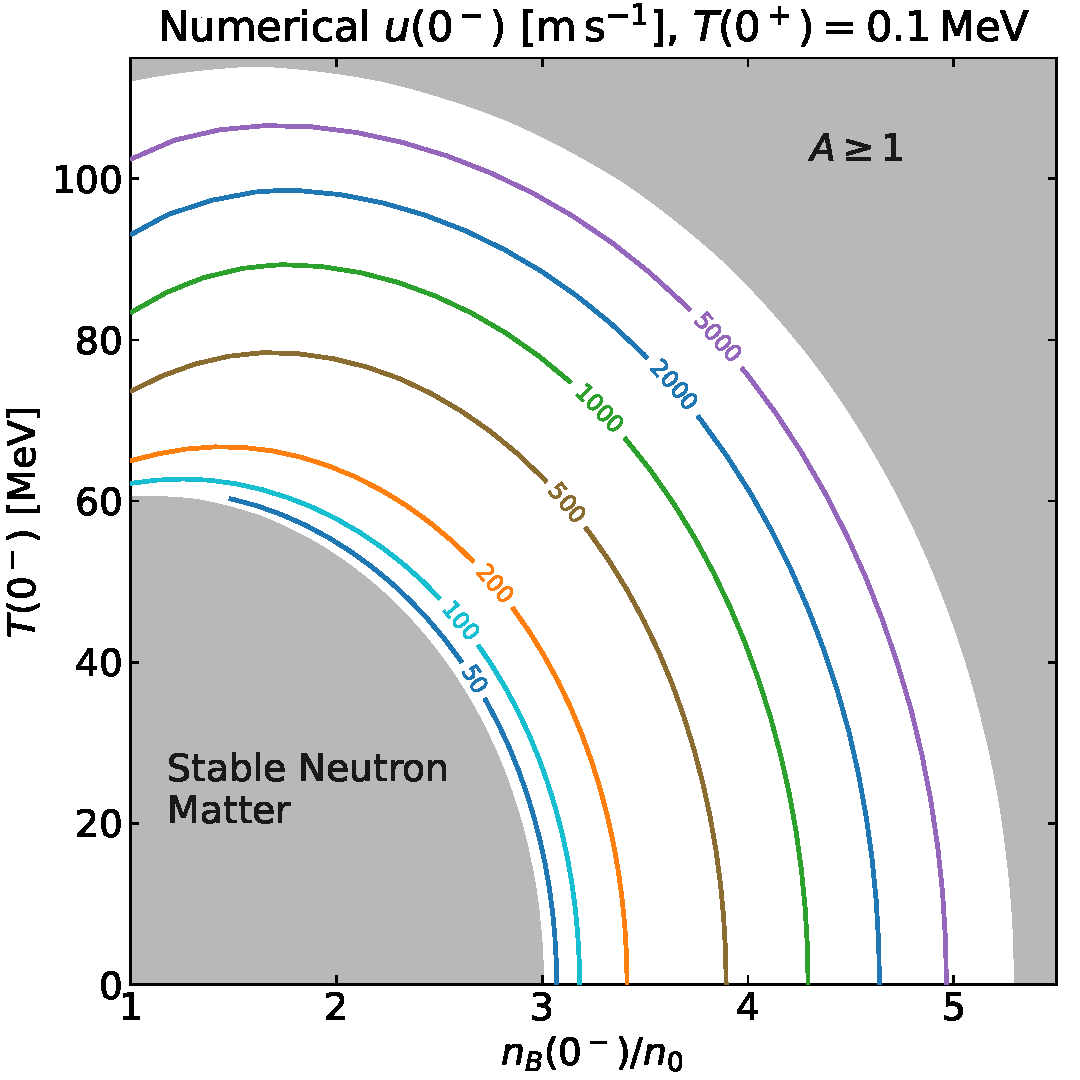
\includegraphics[width=\linewidth]{Plots/Numerical-contour.pdf}
  \caption{
  \LBcom{In the isothermal case does the upper grey region curve back down at high T(0-)? I suspect not.}\JScom{No it doesn't}
  Full numerical phase-boundary speed $u(0^-)$ in $\m\,\s^{-1}$ as a function of the upstream baryon density and temperature, with $T(0^+)=0.1\,\MeV$ and $n_B^{\rm crit}(T{=}0)=3n_0\,.$
  The white band is the domain in which the moving-front solution exists.
  Below the lower boundary neutron matter is stable against the assumed conversion, while the region marked $A\geq1$ lies outside the weak-interaction-limited branch described by our model.
  The contours are drawn at $50\,,$ $100\,,$ $200\,,$ $500\,,$ $1000\,,$ $2000\,,$ and $5000\,\m\,\s^{-1}\,.$}
  \label{fig:numerical}
  % Legacy aliases retained for collaborator notes later in the manuscript.
  \label{fig:u-analytical-loglog}
  \label{fig:T_vs_nB0-}
\end{figure}

%The accepted numerical solutions span speeds from a few tens to a few thousand meters per second.
%At fixed $T(0^-)\,,$ the boundary generally moves faster as $n_B(0^-)$ increases and the state moves away from the lower, zero-speed boundary.
%The speed also rises toward the $A=1$ boundary, but that trend should not be extrapolated into the shaded region, where the assumed weak-interaction-limited branch is no longer applicable.

%The temperature dependence is less simple than in the piecewise-constant estimate.
%Changing $T(0^-)$ changes the location of the zero-speed boundary, the diffusion coefficient, the exact weak rate, and the thermodynamic profile at the same time.
%For example, the zero-speed density decreases from approximately $3.01n_0$ at $T(0^-)=0$ to $1.41n_0$ at $T(0^-)=60\,\MeV\,.$
%Consequently, increasing the temperature at fixed density can move the system farther from the zero-speed boundary and increase the front speed, even though the leading contribution to $D_K$ decreases with temperature.
%The curvature of the contours in Fig.~\ref{fig:numerical} reflects this competition and cannot be inferred from the temperature scaling of $D_K$ alone.

\subsection{Approach to equilibrium}

\begin{itemize}
  \item about the $z(4)$ plot:
  \begin{itemize}
    \item basics, set up, what it means, why we choose that slope 
    \item talk about the plot, the fact that time is over tens of seconds
    \item important: the $z\to 0$ behavior
  \end{itemize}
\end{itemize}

\mgacom{I would like this paper to have a section like the one we had in our previous version, where we calculate the time taken for the boundary to reach its equilibrium position.
Maybe we could add to that some estimate of the impact on gravitational wave signals, but let's discuss this at our next meeting before writing anything more elaborate.}\JScom{Done, see Fig.~\ref{fig:z(t)}}

%We now use the numerical speed map to estimate how long the phase boundary takes to reach the temperature-dependent zero-speed surface.
%Let $z$ be the remaining macroscopic distance to that surface, rather than the microscopic front coordinate $x\,.$
%For each fixed upstream temperature, we assume
%\begin{equation}
% \frac{n_B(0^-;z)}{n_0}
% =\frac{n_{B,0}\bigl(T(0^-)\bigr)}{n_0}
% +\left(0.3\,\km^{-1}\right)z\, ,
% \label{eq:z-density-profile}
%\end{equation}
%where $n_{B,0}\bigl(T(0^-)\bigr)$ is the density on the zero-speed boundary in Fig.~\ref{fig:numerical}.
%We set the initial distance to $z_0=1\,\km\,,$ interpolate $u(0^-)$ along the corresponding constant-$T(0^-)$ path, and integrate $dz/dt=-u(0^-;z)$ with consistent units.
%Thus every curve begins $0.3n_0$ above its own zero-speed density, rather than at the same absolute density.

\begin{figure}
  \centering
  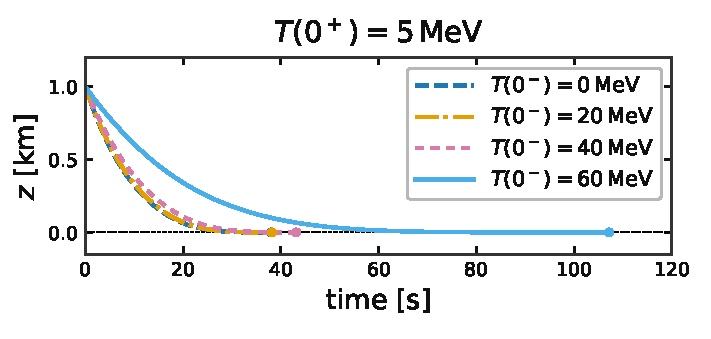
\includegraphics[width=\linewidth]{Plots/z-time-evolution.pdf}
  \caption{Remaining distance $z(t)$ to the zero-speed surface, obtained from the full numerical speed map at fixed $T(0^+)=5\,\MeV\,.$
  The initial distance is $z_0=1\,\km\,,$ and the assumed density gradient is $0.3n_0\,\km^{-1}\,.$
  The points mark the fitted catch-up times for $T(0^-)=0\,,$ $20\,,$ $40\,,$ and $60\,\MeV\,.$}
  \label{fig:z(t)}
\end{figure}

%The catch-up times are $38.1\,,$ $38.2\,,$ $43.2\,,$ and $107.2\,\s$ for $T(0^-)=0\,,$ $20\,,$ $40\,,$ and $60\,\MeV\,,$ respectively.
%The curves therefore reach the zero-speed surface in finite time in all four cases, but the approach becomes much slower at the highest temperature.
%This delay is controlled by the final part of the trajectory, where the front decelerates toward zero speed, rather than by the first kilometer-scale motion alone.
%For the $60\,\MeV$ case, approximately $96\,\s$ of the $107\,\s$ total comes from this near-boundary tail.

%The numerical grid does not extend all the way to the zero-speed surface, so we close the unresolved interval with a power law $u(0^-)\propto z^p$ anchored to the innermost numerical point.
%The fitted exponents lie between $p=0.72$ and $0.81\,,$ which gives a finite integral of $dz/u$ in each case.
%Changing the fit window moves the first three catch-up times into the range $38$--$49\,\s\,,$ while the $60\,\MeV$ result ranges from $107$ to $149\,\s\,.$
%The strong sensitivity of the hottest trajectory is another indication that the late-time slowdown, rather than the speed far from equilibrium, controls the total conversion time.
%These estimates describe a planar laminar front at fixed $T(0^+)\,;$ determining the interface temperature dynamically will require thermal transport across the phase boundary.


\hide{
\subsection{Postmerger gravitational wave peak frequency shift}
\label{sec:gw}


The postmerger gravitational-wave spectrum of a neutron-star merger usually has a single peak at $f_{\rm peak}\approx2$--$4\,\kHz$, which comes from the fundamental quadrupolar ($m=2$) oscillation of the remnant \cite{Stergioulas:2011gd,Takami:2014tva}.
%\AHcom{what does this mean?}\JScom{The index $m$ is the azimuthal mode number.
%A perturbation of a nearly axisymmetric remnant can be expanded in the angle $\phi$ about the rotation axis into terms that vary as $e^{i(m\phi-\omega t)}$, and $m$ counts how many full cycles the pattern completes in one turn around that axis.
%An $m=0$ pattern is axisymmetric, a breathing or quasi-radial motion; $m=1$ is a one-sided displacement; $m=2$ stretches the equatorial cross-section into a rotating bar.
%Only the bar radiates appreciably.
%Gravitational-wave emission has no monopole or dipole part, so it comes from the mass quadrupole, and within the quadrupole the $m=2$ component has a time-varying moment while the $m=0$ (axisymmetric) component does not.
%Strictly, $m$ fixes only the azimuthal shape: the dominant peak is the $\ell=m=2$ fundamental mode, with smaller $m=2$ contributions from higher multipoles $\ell=3,4,\dots$
%A pattern $\propto e^{i(2\phi-\omega t)}$ rotates rigidly at angular speed $\omega/2$ and looks the same after half a turn, so a distant observer sees the quadrupole repeat twice per revolution and the wave emerges at $f_{\rm peak}=\omega/2\pi\ $.}
Simulations find that compared with purely hardronic matter, having an instantaneous first-order transition to quark matter would shifts $f_{\rm peak}$ by several hundred Hz \cite{Bauswein:2018bma,Most:2018eaw,Weih:2019xvw,Bauswein:2020ggy,Fujimoto:2022xhv,Espino:2023llj}.
All of these simulations convert nuclear matter the instant its pressure exceeds $p_\text{crit}$, which is the instantaneous-conversion described in the introduction.
Here we estimate how the finite phase boundary speed obtained in Sec.~\ref{sec:results} changes that prediction.
We write $f_{\rm peak}^{\infty}$ for the peak frequency under instantaneous conversion and $f_{\rm peak}^{\rm finite}$ for the peak frequency when the nuclear to quark phase transition is limited by boundary propagation speed we calculated.

\textbf{Quark matter fraction under a finite-speed conversion.}
At each time $t$, we define region where quark matter is thermodynamically favored by
\begin{equation}
\Omega_{\rm crit}(t)
=\left\{\boldsymbol{x}:\,P(\boldsymbol{x},t)>p_\text{crit}\right\},
\label{eq:critical_region}
\end{equation}
with $p_\text{crit}$ determined as in Sec.~\ref{sec:results}.
Under the instantaneous conversion assumption all of $\Omega_{\rm crit}$ is quark matter.
With a finite conversion speed, metastable nuclear matter in $\Omega_{\rm crit}$ converts only after the phase boundary has swept over it, which we track with an indicator field $I_q(\boldsymbol{x},t)$: $I_q=1$ where there's deconfined quark matter and $I_q=0$ elsewhere.
Matter with $P>p_\text{crit}$ and $I_q=0$ is the metastable nuclear matter whose conversion speed we calculated in Sec.~\ref{sec:speed}.
%We assume that converted matter stays converted if the local pressure later falls back below $p_\text{crit}$.

%The motion of the boundary in the merger frame follows from Sec.~\ref{sec:speed}.
%The front advances into the nuclear matter at speed $u(0^-)$ relative to nuclear matter, so the boundary moves with the local fluid velocity plus $u(0^-)$ along the boundary's normal direction, towards the nuclear phase.
%For merger relavant temperature $\leq 50$ MeV and metastability, the calculated speeds obey $u(0^-)\lesssim10^{-5}$ in natural units, so we do not distinguish between proper and ordinary 3-velocity in this section.
%Advection by the merger flow rearranges the boundary but does not convert nuclear matter; the converted volume grows only through the normal propagation at $u(0^-)$.
%In a simulation, $I_q$ can be implemented as a marker (level-set) field transported with this velocity; Appendix~\ref{sec:finite_rate_implementation} gives the prescription.

We measure the progress of conversion by the converted volume fraction of the critical-pressure region $\Omega_{\rm crit}\ $,
\begin{equation}
X_q(t)
=\frac{1}{V_{\rm crit}(t)}
\int_{\Omega_{\rm crit}(t)}I_q(\boldsymbol{x},t)\,dV\,,
\label{eq:converted_fraction}
\end{equation}
where $V_{\rm crit}(t)$ is the volume of $\Omega_{\rm crit}(t)\ $.
%The same definition can be weighted by baryon density, or by the local sensitivity of the $m=2$ mode to the equation of state, without changing the estimates below.
Evaluating $X_q$ requires a geometry for $\Omega_{\rm crit}\ $, which is natural known for a simulation, but we approximate the merger shape by a sketch in Fig.~\ref{fig:omega_crit_geom}.
We assume that each of the two inspiraling neutron stars already has a quark-matter core of radius $R_0$, which depends on the initial star masses.
When the stars merge, the remnant keeps a double-core structure for the first few milliseconds, \JScom{Is the quark core rigid enough to keep the shape of a sphere?} so in the equatorial plane $\Omega_{\rm crit}$ splits into two congruent lobes that wrap around one another, making a taichi shape with one of the original stellar cores, at the center of each lobe.
This is the same $m=2$ deformation that carries the mass quadrupole responsible for the postmerger GW emission, so the converted fraction and its mode-weighted variant refer to the same region.
The pattern corotates with the fluid, so rotation carries the lobes around without converting any matter.
The two quark cores that the stars bring in are the seeds, and we are not considering strange quark matter nucleation here.
Each core boundary then advances into the surrounding metastable nuclear matter at speed $u(0^-)$, so over the postmerger emission window $\Delta t_{\rm pm}$ the core radius grows from $R_0$ to $R_0+u(0^-)\,\Delta t_{\rm pm}$, and
\begin{equation}
X_q
=
\left[\frac{R_0+u(0^-)\,\Delta t_{\rm pm}}{R_{\rm lobe}}\right]^{3}
\,,\quad X_q \leq 1
\label{eq:lobe_fraction}
\end{equation}
where $R_{\rm lobe}\equiv[3V_{\rm crit}/(8\pi)]^{1/3}$ is the effective radius of one lobe and $V_{\rm crit}$ the total volume of $\Omega_{\rm crit}$.
The pre-merger cores set the baseline $X_q(\Delta t_{\rm pm}{=}0)=(R_0/R_{\rm lobe})^3$.
The part the front adds is a thin shell: for $u(0^-)\,\Delta t_{\rm pm}\ll R_0$ each core gains a volume $4\pi R_0^{2}\,u(0^-)\,\Delta t_{\rm pm}$, linear in the front speed rather than cubic.

\begin{figure}[t]
  \centering
  \IfFileExists{Plots/omega_crit_taiji_3d.pdf}{%
    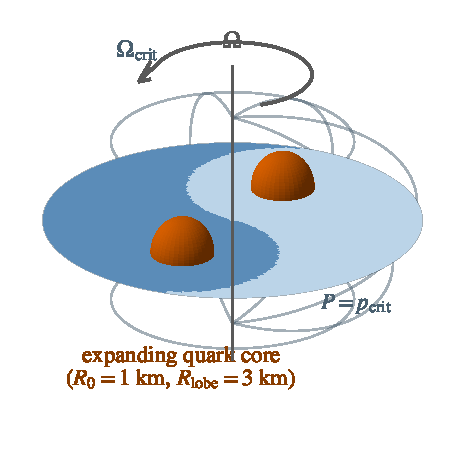
\includegraphics[width=1\columnwidth]{Plots/omega_crit_taiji_3d.pdf}%
  }{%
    \includegraphics[width=1\columnwidth]{omega_crit_taiji_3d.pdf}%
  }
  \caption{Geometry of the critical-pressure region $\Omega_{\rm crit}$ in the early remnant.
  The cage of rings is the $P=p_{\rm crit}$ surface of the oblate remnant core.
  The equatorial cut shows the two congruent lobes of the rotating $m=2$ double-core pattern (taiji shape); the two tones only distinguish the lobes, which hold the same metastable nuclear matter.
  Each lobe carries one of the pre-merger quark cores (shaded spheres, drawn to scale for $R_0=1\,\km$ and $R_{\rm lobe}=3\,\km$).
  Over the emission window the conversion front advances each core boundary by only $u(0^-)\,\Delta t_{\rm pm}\approx10\,\m$.}
  \label{fig:omega_crit_geom}
\end{figure}

\textbf{Catch-up within the emission window.}
$f_{\rm peak}^{\rm finite}$ meets $f_{\rm peak}^{\infty}$ only if the front reaches every point of $\Omega_{\rm crit}$ within that window. 
And to achieve this, the front velocity $u(0^-)$ should satisfy:
\begin{equation}
u(0^-)\gtrsim\frac{L_{\rm max}}{\Delta t_{\rm pm}}
\quad\Longrightarrow\quad
f_{\rm peak}^{\rm finite}\simeq f_{\rm peak}^{\infty}\,,
\label{eq:catch_up}
\end{equation}
where $L_{\rm max}$ is longest diatance the phase boundary has to swipe over to convert the entire $\Omega_{\rm crit}$ to quark matter. %largest propagation distance, measured through the matter, from the initial seed surface to any point of $\Omega_{\rm crit}$.

Both sides of Eq.~\eqref{eq:catch_up} are fixed by known numbers.
Quark cores in instantaneous-conversion simulations extend over a few kilometers \cite{Most:2018eaw,Bauswein:2018bma}; as reference values we take the radius of merger medium with pressure greater than $p_{\rm crit}$ to be $R_{\rm lobe}=3\,\km$ and each merging neutron star has a quark core of radius $R_0=1\,\km$, and the postmerger peak is accumulated over $\Delta t_{\rm pm}\approx5$--$20\,\text{ms}$ of emission \cite{Takami:2014tva,Vretinaris:2019spn}.
The the core boundary is the phase boundary, and the farthest matter sits at the tip of the wrapping tail, so $L_{\rm max}\approx2R_{\rm lobe}-R_0\approx5\,\km$ and catching up requires $u(0^-)\gtrsim3\times10^{5}$--$10^{6}\,\m\,\s^{-1}$.
The maximum boundary speeds of Sec.~\ref{sec:results} at merger temperatures, $u_{\rm max}(0^-)\approx10^{2}$--$10^{3}\,\m\,\s^{-1}$, fall short by factors of $300$ to $10^{4}$.
This is the quantitative form of the concern raised in the introduction: the instantaneous conversion implicitly assumes boundary speeds at least $10^{6}\,\m\,\s^{-1}$, while weak-interaction-limited propagation reaches at most $10^{3}\,\m\,\s^{-1}$.
The front therefore barely moves the converted fraction.
For $u(0^-)\sim 10^{3}\,\m\,\s^{-1}$ and $\Delta t_{\rm pm}\sim 10\,\text{ms}$ each core radius grows by $\sim 10\,\m$, which is about one percent of $R_0$, and Eq.~\eqref{eq:lobe_fraction} moves $X_q$ only from the baseline $(R_0/R_{\rm lobe})^3=0.037$ to $0.038$.

On the timescale of the postmerger emission, weak-interaction-limited conversion is frozen: the phase boundary is a comoving surface, and outside the two quark matter cores $\Omega_{\rm crit}$ stays metastable nuclear matter.
Interface-mode analyses of the inspiral assume the same frozen composition \cite{Tonetto:2020bie,Counsell:2025hcv,Pereira:2025xsi}; here it follows from the microphysics under merger conditions.
Converting the whole core within the window would instead need seeds spread through the volume, spaced by no more than $\sim2\,u_{\rm max}(0^-)\,\Delta t_{\rm pm}\approx20\,\m$.
Whether nucleation can supply that seed density is a question of bubble-nucleation physics rather than boundary propagation, and we do not address it here.
Hydrodynamic instabilities of the front could also raise the effective conversion rate above our planar bound, as discussed in Sec.~\ref{sec:conclusion}.

\textbf{Peak-frequency shift and observability.}
Let $\Delta f_{\rm PT}$ denote the signed shift of the peak frequency between a remnant whose critical-pressure region $\Omega_{\rm crit}$ is fully converted and one that is purely metastable nuclear matter, so:
\begin{equation}
\Delta f_{\rm PT}\equiv f_{\rm peak}^{\infty}-f_{\rm peak}(X_q{=}0)
\label{eq:Delta_f_PT}
\end{equation}
%Note that we assume the two stars come with quark cores, so in this case, $X_q\geq (R_0/R_{\rm lobe})^3\ $.
Under the instantaneous-conversion assumption of the existing simulations $\Delta f_{\rm PT}$ is an equilibrium quantity fixed by the equation of state: a pure nuclear matter EoS run gives $f_{\rm peak}(X_q{=}0)$, and a hybrid EoS run that switches to quark matter above $p_{\rm crit}$ gives $f_{\rm peak}^{\infty}$.
Such simulations find $|\Delta f_{\rm PT}|$ of several hundred Hz for strong first-order transitions \cite{Bauswein:2018bma,Most:2018eaw,Weih:2019xvw,Prakash:2023afe}.
$\Delta f_{\rm PT}$ can also be read off observationally, as a deviation of $f_{\rm peak}$ from hadronic empirical relations of the form $f_{\rm peak}^{\infty}=F(\mathcal{M}_{\rm chirp},R_{1.8})$, where $\mathcal{M}_{\rm chirp}$ is the chirp mass and $R_{1.8}$ the radius of a cold, nonrotating $1.8\,M_\odot$ star \cite{Bauswein:2012ya,Vretinaris:2019spn}.
However, we assume the two stars come with quark cores, so in this case, $X_q\geq (R_0/R_{\rm lobe})^3\ $, and never goes to zero.

To place the finite-rate peak frequency $f_{\rm peak}^{\rm finite}$ between $f^\infty_{\rm peak}$ and $f_{\rm peak}(X_q{=}0)$, we argue that the peak frequency shifts, given by 
\begin{equation}
\Delta f_{\rm peak} = f^{\infty}_{\rm peak} - f^{\rm finite}_{\rm peak}
\label{eq:Delta_f_peak}
\end{equation}
and the reference $\Delta f_{\rm PT}$ are related by the converted fraction $X_q$.
Converting a volume element replaces nuclear matter by quark matter, which changes the local pressure-density relation and therefore the restoring force and inertia of the mode.
For a small converted volume these shifts add over the converted region, so if the mode has roughly uniform sensitivity across $\Omega_{\rm crit}$ the frequency moves in proportion to $X_q$,
\begin{equation}
\begin{aligned}
f_{\rm peak}^{\rm finite}
&\simeq
f_{\rm peak}(X_q{=}0)+X_q(\Delta t_{\rm pm})\,\Delta f_{\rm PT}
\\
&=
f_{\rm peak}^{\infty}-\bigl[1-X_q(\Delta t_{\rm pm})\bigr]\,\Delta f_{\rm PT}\,,
\end{aligned}
\label{eq:finite_peak_frequency}
\end{equation}
where $X_q$ is the total quark-matter fraction inside $\Omega_{\rm crit}$, including the pre-merger quark cores.
To better understand this, if $X_q = 0$, which means there's no quark matter, and the two stars don't even have quark cores to begin with. 
In this case, $\Delta f_{\rm peak} = \Delta f_{\rm PT}$, but we know from Eq.~\eqref{eq:lobe_fraction} that $X_q\geq (R_0/R_{\rm lobe})^3$ since we assume that the two stars have quark cores.
On the other hand, if $X_q = 1$, which means all matter in $\Omega_{\rm crit}$ is converted to quark matter, then $f_{\rm peak}^{\rm finite} = f_{\rm peak}^{\infty}\ $, and $\Delta f_{\rm peak} = 0\ $.

The linear law is a leading-order approximation; terms nonlinear in $X_q$ describe higher-order changes in the mode structure and need simulations at intermediate converted fractions.
%Because the cores sit at the lobe centers, where the $m=2$ bar has its largest amplitude, their weight in the mode may exceed their volume fraction, so $X_q(u{=}0)\,\Delta f_{\rm PT}$ is a lower estimate of their contribution.
Subtracting Eq.~\eqref{eq:finite_peak_frequency} from $f_{\rm peak}^{\infty}$ gives:
\begin{equation}
\Delta f_{\rm peak}
\equiv
f_{\rm peak}^{\infty}-f_{\rm peak}^{\rm finite}
\simeq
\bigl[1-X_q\bigr]\,\Delta f_{\rm PT}\,.
\label{eq:rate_shift}
\end{equation}
Two effects set porportionality relation, and only one of them is the front speed.
The pre-merger cores already fill a fraction $X_q(\Delta t_{\rm pm}{=}0)=(R_0/R_{\rm lobe})^3=0.037$ of $\Omega_{\rm crit}$, which by itself leaves a deficit $[1-X_q(u{=}0)]\,\Delta f_{\rm PT}\approx0.96\,\Delta f_{\rm PT}$.
Over the emission window the finite front adds only $\Delta X_q\approx10^{-3}$ to $X_q$, a further shift of $\Delta X_q\,\Delta f_{\rm PT}\approx0.1$--$0.9\,$Hz.
The slow front is therefore dynamically frozen, and the large deficit reflects the small size of the pre-merger cores rather than the front speed.

Figure~\ref{fig:rate_deficit} shows $\Delta f_{\rm peak}$ as a function of the boundary speed, for six values of $\Delta f_{\rm PT}$ calibrated as endpoint differences from published instantaneous-conversion simulations \cite{Prakash:2023afe,Bauswein:2018bma}.
Across the calculated $u_{\rm max}(0^-)\approx10^{2}$--$10^{3}\,\m\,\s^{-1}$ the peak frequency shift stays near $0.96\,\Delta f_{\rm PT}$, so the shift predicted by instantaneous-conversion simulations is not realized and the instantaneous prescription misplaces the peak by nearly the full $|\Delta f_{\rm PT}|$.

\begin{figure}
  \centering
  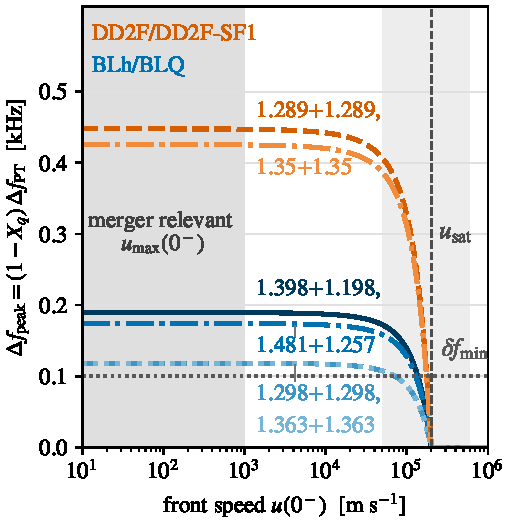
\includegraphics[width=\columnwidth]{Plots/f_peak.pdf}%
  \caption{Finite-rate frequency deficit $\Delta f_{\rm peak}=(1-X_q)\,\Delta f_{\rm PT}$ from Eqs.~\eqref{eq:lobe_fraction} and \eqref{eq:rate_shift}, using the pre-existing-core geometry with $R_0=1\,\km$, $R_{\rm lobe}=3\,\km$, and $\Delta t_{\rm pm}=10\,\text{ms}$.
  Each curve uses a $\Delta f_{\rm PT}$ calibrated as the endpoint difference between hybrid-EOS and purely hadronic instantaneous-conversion simulations, labeled by EOS pair and binary masses; five cases (all BLh/BLQ pairs and the DD2F/DD2F-SF1 $1.289{+}1.289$ pair) are from Table IV of \cite{Prakash:2023afe}, and the DD2F/DD2F-SF1 $1.35{+}1.35$ pair is from \cite{Bauswein:2018bma}.
  The two BLh/BLQ binaries with $\Delta f_{\rm PT}=0.123\,\kHz$ overlap.
  Neither reference reports the size of the quark-matter region, so we apply the same fiducial geometry to all six cases.
  The converted fraction $X_q(u(0^-))$ is then common to every curve and $\Delta f_{\rm PT}$ only rescales it, which is why the curves fall off together: the location of the fall-off is set by the geometry alone, not by the equation of state.
  The grey band on the left marks the maximum boundary speeds calculated in Sec.~\ref{sec:results} at merger temperatures.
  The dashed line is the saturation speed $u_{\rm sat}=(R_{\rm lobe}-R_0)/\Delta t_{\rm pm}$, above which the front would fill the lobes within the emission window, and the light band around it shows how far $u_{\rm sat}$ moves for $R_{\rm lobe}=2$--$4\,\km$ and $\Delta t_{\rm pm}=5$--$20\,\text{ms}$.
  Throughout the shaded band the deficit is $(1-X_q)\,\Delta f_{\rm PT}\approx0.96\,\Delta f_{\rm PT}=0.12$--$0.45\,\kHz$, above the $\delta f_{\rm min}\approx0.1\,\kHz$ resolution of a loud (postmerger signal-to-noise ratio ${\gtrsim}10$) next-generation detection \cite{Breschi:2022ens,Clark:2015zxa}.}
  \label{fig:rate_deficit}
\end{figure}

Whether this is detectable depends on the frequency resolution of postmerger observations.
The discrepancy is measurable if
\begin{equation}
\bigl[1-X_q\bigr]\,\bigl|\Delta f_{\rm PT}\bigr|
\gtrsim\delta f_{\rm min}\,,
\label{eq:observability}
\end{equation}
where $\delta f_{\rm min}$ is the smallest resolvable shift of the peak.
This resolution depends heavily on how loud the postmerger signal is.
For the Einstein Telescope, Bayesian recoveries of the peak frequency carry errors of order $1\,\kHz$ at postmerger signal-to-noise ratio $7$, roughly the detection threshold, but tighten to below $0.1\,\kHz$ at signal-to-noise ratio $10$ \cite{Breschi:2022ens}.
A Fisher estimate for a nearby source at ${\sim}30\,$Mpc with advanced LIGO gives a similar scale, $\delta f_{\rm peak}\approx50\,$Hz \cite{Clark:2015zxa}.
Bayesian model selection can distinguish phase-transition-induced shifts of this size \cite{Prakash:2023afe}.
We therefore take $\delta f_{\rm min}\approx0.1\,\kHz$ as the resolution of a loud postmerger detection.
The calibrated $|\Delta f_{\rm PT}|$ span $0.12$--$0.47\,\kHz$ and $1-X_q\approx0.96$, so the deficits are $0.12$--$0.45\,\kHz$ (Fig.~\ref{fig:rate_deficit}).
Equation~\eqref{eq:observability} then holds for every case once the postmerger signal-to-noise ratio reaches ${\sim}10$, while near the detection threshold the ${\sim}1\,\kHz$ errors would hide all of them.
A detected postmerger peak from a remnant that crosses the transition should therefore sit at the metastable hadronic value rather than at the shifted equilibrium value, unless nucleation seeds conversion densely enough to bypass the front-speed bound.

The inputs to this estimate (the geometry of $\Omega_{\rm crit}$, the emission window $\Delta t_{\rm pm}$, and the calibration $\Delta f_{\rm PT}$) all depend on the binary chirp mass, so Eqs.~\eqref{eq:finite_peak_frequency} and \eqref{eq:observability} define $f_{\rm peak}^{\rm finite}(\mathcal{M}_{\rm chirp},u(0^-))$ once those inputs come from equilibrium sequences or from numerical relativity.
We do not predict the strain amplitude of the peak; that requires the excitation energy and damping of the $m=2$ mode in addition to its frequency.
}




\section{Conclusion}
\label{sec:conclusion}
\begin{itemize}
    \item Impact of instabilities, Urca processes, ... on phase boundary speed
\end{itemize}
\AH{Our results allow us to speculate on the fate of interface modes in the inspiral. Typical frequencies of interface modes depend on the EoS of nuclear and quark matter as well as the star's mass, where heavier stars show lower frequency resonances. The frequencies themselves range from a couple hundred to around $f=2000$ Hz (see Fig.~2 of Ref.~\cite{Counsell:2025hcv}). Depending on the energy absorbed by the mode, the amplitude ranges from a few millimeters to centimeters in the inspiral, and might reach several meters in the postmerger. Assuming a frequency of $f=700$ Hz, we can calculate the resonant velocity where the timescale of the oscillation matches the time given by the amplitude divided by the phase boundary velocity. In this resonant scenario, we expect viscous effects as described in \cite{Alford:2014jha} become important. At even larger velocities, we expect the mode to lose its support (see discussion in the nuclear case in Ref.~\cite{Zhao:2025pgx}) and vanish. In the inspiral, the resonant velocity ranges from $v_\text{res}=1$ m$/$s to $v_\text{res}=15$ m$/$s, which is within the range found in our calculation shown in Fig.~\ref{fig:u-analytical-loglog}. In the postmerger scenario, the resonant velocity rises to $\mathcal{O}(1000\, \text{m/s})$, which is reached in the strongly metastable scenario (see Fig.~\ref{fig:T_vs_nB0-}). This shows that any accurate calculation of the interface mode must include the finite phase boundary velocity and viscous effects, potentially via the dynamical sound-speed formalism developed in Ref.~\cite{Zhao:2025pgx} and applied to quark matter in \com{cite Zhao Han Haber}.

This also motivates a more detailed calculation of the phase boundary velocity:
\begin{itemize}[leftmargin=*]
    \item In this paper, we model the baryonic side as pure neutron matter. However, in compact stars, baryonic matter is composed of chemically equilibrated nuclear matter, which includes not only neutrons, but also protons, electrons, and muons in a composition determined by charge neutrality and chemical equilibration. Even hyperonic matter could be considered on the baryonic side of the phase boundary.
    \item The presence of leptonic particles opens up the possibility of proton or strangeness-changing Urca rates. The phase boundary velocity would then potentially be slowed down even further, as we now need to equilibrate multiple particle fractions on the quark matter side via the generally slower Urca processes. Our results thus likely present an upper bound on the velocity.
    \item At high temperatures, the physics of neutrinos might become important as neutrinos could cool down the conversion region, or if they get trapped, will alter the hydrodynamic description of the phase boundary. However, given our recent work in Refs.~\cite{Alford:2025jtm,Alford:2026kwd}, neutrino trapping on the microscopic scale of the phase boundary seems unfeasible, but could potentially play a role in the equilibrated baryonic or quark matter
    \item At the temperatures occurring in the inspiral, baryonic and quark matter might be found in a (color-)superconducting/superfluid state. Cooper pairing will not only alter the hydrodynamics of the problem, but suppresses the flavor-changing rates used in this work, and will also alter diffusive transport, thus furder slowing down the phase boundary.
    \item In this work, we have assumed that thermal equilibration across the phase boundary is happening on a timescale slower than the evolution of the phase boundary. Towards the end of the equilibration process, however, the phase boundary slows down (\AHcom{do we have a section explaining this?}. To not only reach flavor, but also thermal equilibration, thermal equilibration across the boundary has to be taken into account. Otherwise, the final state of the evolution will be wrongly described as a state where the baryonic and the quark matter phase stay at different temperatures.

    \item In this work, we assume that all profiles on the nuclear matter side are constant, and neglect any disturbance propagating ahead of the phase boundary. 
    \item Furthermore, the assumption of a steady state, which we deem reasonable, should be further investigated.
    \item Our hydrodynamic description is based on an ideal fluid description. Dissipative corrections might be taken into account in the stress-energy tensor, or be included via weak interactions as described in Ref.~\cite{Most:2022yhe}.
        \item If the phase boundary is driven by large-scale oscillations (as we expect it in the inspiral and the merger), the opposite scenario, where quark matter recombines to nuclear matter, has to be calculated. This will also allow us to estimate the strength of the so-called "phase conversion dissipation", a dissipative effect stemming from the out-of-phase movement of the actual phase boundary with the critical pressure \cite{Alford:2014jha}.
        \item Cooper pairing: influence on diffusion, weak interaction rates, anything else?
        \item surface tension?
\end{itemize}
}
\section*{Acknowledgements} We thank XXX (Nils Andersson? Suprovo Ghosh?) for valuable feedback and discussions.
MGA, LB, and AH are partly supported by the U.S. Department of Energy, Office of Science, Office of Nuclear Physics, under Award No.~\#DE-FG02-05ER41375. A.H.~furthermore acknowledges financial support by the UKRI under the Horizon Europe Guarantee project EP/Z000939/1.


\appendix
\section{Bag model of quark matter}
\label{sec:bag_model}

\mgacom{If we decide to impose electrical neutrality then this will need some rewriting.}
In the approximation that we use for quark matter, ignoring electromagnetism and leptons, the pressure of quark matter is the sum of the pressures of the individual flavors,
\begin{equation}
\begin{array}{rl}
 P_\text{QM}(\mu_q,\mu_K,T) &= P_q(\mu_q,T)
 + P_q(\mu_q{+}\mu_K/2,T)  \\[1ex]
  & +\ P_q(\mu_q{-}\mu_K/2,T) - U_\text{bag} \ ,
\end{array}
%  \dfrac{1}{32\pi^2}\bigl( 24\mu_q^4 + 24 \mu_q^2\mu_K^2 + \mu_K^4\bigr) 
 \label{eq:QM-bag-EoS}
\end{equation}
where $\mu_q=\mu_B/3$ is the quark chemical potential and $P_q$ is the pressure of a free Fermi gas of three colors of a single quark flavor. In this approximation the individual flavors have chemical potentials $\mu_u=\mu_B/3$, $\mu_d =\mu_B/3 + \mu_K/2$, and $\mu_s= \mu_B/3 - \mu_K/2$. We expect $\mu_K,T \ll \mu_q$ so we expand in powers of these to obtain
\begin{equation}
\begin{aligned}
P_{\text{QM}} & =
-U_\text{bag}+\frac{\mu_B^4}{108\pi^2}
+
\frac{\mu_B^2}{12\pi^2}\mu_K^2
+
\frac{\mu_K^4}{32\pi^2}\\[1ex]
& +
\frac{\mu_B^2}{6}T^2
+
\frac{1}{4}\mu_K^2T^2
+
\frac{19\pi^2}{36}T^4
+\cdots ,
\end{aligned}
\label{eq:Qm-EoS-4th-order}
\end{equation} 
\mgacom{Do we use this 4th order form of the EoS anywhere?}\JScom{No, we never use it again: only the quadratic truncation \eqref{eq:QM-EoS-2nd-order} is cited later (line~480 and the analytic derivation in Sec.~\ref{sec:hydro_analytic}). Worth keeping, though: these are exactly the terms we'd need if we later want to estimate how far the analytic formula should deviate from the full numerical result, since they're what the quadratic truncation drops. We don't have that comparison anywhere in Sec.~\ref{sec:results} yet.}
or to quadratic order,
\begin{equation}
 P_{\text{QM}} = -U_\text{bag}+\frac{\mu_B^4}{108\pi^2}
+
\frac{\mu_B^2}{12\pi^2}\mu_K^2
 +\frac{\mu_B^2}{6} T^2\,,
 \label{eq:QM-EoS-2nd-order}
\end{equation}
which implies that to leading order,
\begin{align}
 n_K & =\dfrac{\partial P_{\rm QM}}{\partial\mu_K}\biggr|_{\mu_B,T} =
\frac{\mu_B^2\mu_K}{6\pi^2}\,,
\label{eq:nK-approx}
 \\[2ex]
 n_B &=\dfrac{\partial P_{\rm QM}}{\partial\mu_B}\biggr|_{\mu_K,T} = \dfrac{\mu_B^3}{27\pi^2} 
 %+ \dfrac{\mu_B \mu_K^2}{6\pi^2} +  \dfrac{\mu_B T^2}{3} 
 \,.
 \label{eq:nB-approx}
\end{align}

We can also express the quark matter properties in terms of the K fraction $a$. To this order,
\begin{equation}
a\equiv\dfrac{n_K}{n_B}=\dfrac{9\mu_K}{2\mu_B} = \dfrac{3\mu_K}{2\mu_q}\,.
\label{eq:a-muK}
\end{equation}

% Equilibrated quark matter satisfies $\mu_K=0\,,$ 

\section{Strangeness creation}
\label{sec:K-creation}

For positive $\mu_K\,,$ the nonleptonic process relaxes the K density at the
rate~\cite{Madsen:1993xx}
\begin{equation}
 \Gamma_K(\mu_B,\mu_K,T)
 =\mathcal A_K\mu_u^5\mu_K
 \left(\mu_K^2+4\pi^2T^2\right)\,,
\label{eq:exact_rate}
\end{equation}
\JScom{$u$ is a real participant, not an average: the reaction is $d+u\leftrightarrow u+s$ (Eq.~\eqref{eq:nonleptonic}), with $u$ a spectator on both sides, like the spectator nucleon in modified Urca. Madsen's rate has the same $\mu_u^5$ prefactor for the same reason.}\mgacom{In that case one would expect factors of $\mu_d$ and $\mu_s$ as well. I think Madsen is using $\mu_u$ as a symbol for something else, probably some average of chemical potentials. In our calculation everything should end up as a function of $\mu_B$, $\mu_K$, and $T$.}
where
\begin{equation}
 \mathcal A_K=
 \frac{16}{5\pi^5}G_F^2
 \sin^2\theta_C\cos^2\theta_C\,,
\label{eq:exact_prefactor}
\end{equation}
where $G_F=1.16637\times10^{-11}\,\MeV^{-2}$ is the Fermi constant and $\theta_C=13.02^\circ$ is the Cabibbo angle.
We use
$\mu_u=\mu_B/3+2\mu_Q/3\,,$ where electric charge chemical potential $\mu_Q$ is fixed by charge neutrality,
$2n_u-n_d-n_s=0\,.$ \mgacom{But in the previous section we said $\mu_u=\mu_B/3$. Which are we actually using? Anyway, as noted above $\mu_u$ shouldn't be needed.}
\JScom{Both, in different places: the exact rate used in the numerical code uses the full $\mu_u=\mu_B/3+2\mu_Q/3$ with $\mu_Q$ solved exactly from charge neutrality, while only the analytic approximation in Sec.~\ref{sec:hydro_analytic} drops $\mu_Q$ and uses $\mu_u\simeq\mu_q$. Not an inconsistency, just two different calculations.} \mgacom{(1) In general we should show the same formulas that we use in the numerical calculation. If we are making some approximation beyond the ones we use in our numerics then we should say so explicitly. (2) In Appendix A we didn't impose electric neutrality. Our overall approach is to ignore electrons and electromagnetism, so it seems inconsistent to impose electric neutrality.}

\hide{
For massless quarks, at leading order in $\mu_K/\mu_q$ and $T/\mu_q\,,$ where $\mu_q=\mu_B/3\,,$ the charge-neutral quark equation of state gives
\begin{equation}
 \mu_u\simeq\mu_q\,,
 \qquad
 n_B\simeq\frac{\mu_q^3}{\pi^2}\,,
 \qquad
 \mu_K\simeq\frac{2}{3}\mu_q a\,.
\label{eq:cubic_rate_expansion}
\end{equation}
Substituting Eq.~\eqref{eq:cubic_rate_expansion} into the exact rate in Eqs.~\eqref{eq:exact_rate} and \eqref{eq:exact_prefactor}, and retaining the leading cubic and thermal-linear terms, gives
\begin{subequations}
\label{eq:cubic_rate}
\begin{align}
 \Gamma_K(n_K,T)
 &=n_B\gamma_K\left(a^3+\eta a\right)\,,
 \qquad
 \eta=\frac{9\pi^2T^2}{\mu_q^2}\,,
\label{eq:source}\\
 \gamma_K
 &=\frac{128}{27\times5\pi^3}
 G_F^2\sin^2\theta_C\cos^2\theta_C\,\mu_q^5\,.
\label{eq:gammaK}
\end{align}
\end{subequations}
}

For the analytic approximation in Sec.~\ref{sec:hydro_analytic}, we use the quadratic approximation of Sec.~\ref{sec:bag_model} to express the rate
in terms of the K fraction. Using \eqref{eq:a-muK},
\begin{equation}
\begin{array}{rl}
 \Gamma_K(a,T) &=n_B\gamma_K\left(a^3+\eta a\right)\,, \\[1ex]
 \gamma_K &= \dsp\frac{128}{27\times5\pi^3}
 G_F^2\sin^2\theta_C\cos^2\theta_C\,\mu_q^5\,, \\[2ex]
 \eta &= \dfrac{9\pi^2 T^2}{\mu_q^2} \,.
\end{array} \label{eq:cubic_rate}
\end{equation}


\section{Strangeness diffusion}
\label{sec:K-diffusion}

The diffusion of the K flavor in quark matter is described by a diffusion coefficient $D_K$, which, since the quarks are relativistic, is closely related to the mean free path.
This is determined by strong interactions, so we model it using
the single gluon exchange perturbative expression \cite{Haensel:1992zz,Heiselberg:1993cr}
\begin{equation}
 D_K^{-1}
 =
 \frac{8N_f\alpha_s^2}{\pi}
 \left(
 h_D\frac{T^{5/3}}{q_D^{2/3}}
 +\frac{\pi^3T^2}{12q_D}
 \right)\,,
\label{eq:diffusion_coefficient}
\end{equation}
Here $N_f=3$ is the number of active quark flavors, $\alpha_s=0.3$ is the strong coupling, $h_D = \Gamma(\frac{8}{3})\zeta(\frac{5}{3})(2\pi)^{2/3} \simeq1.81$ is a numerical prefactor, $q_D$ is the
Debye wavenumber defined by $q_D^2=g^2N_f\mu_q^2/(2\pi^2)\,,$ and $g^2=4\pi\alpha_s\,.$ 
In our numerical calculations we set $\al_s=0.3$
\mgacom{Can we find some standard citation about the running of the QCD coupling that would show that this is an appropriate value at energy scales of order $400\,\MeV$?}\JS{\cite{Farhi:1984qu,Madsen:1998uh}}\ .

In \eqref{eq:diffusion_coefficient} the first term comes from the interaction mediated by Landau-damped transverse gluons, and the second term comes from Debye-screened longitudinal \mgacom{and transverse?} gluons. The first term is larger at temperatures up to $0.5 \sqrt{\al_s}\mu_q$ which is of order $70\,\MeV$, but because both terms have such similar $T$ dependence they are already of comparable size (to within at factor of 2) when the temperature rises above $0.04 \sqrt{\al_s}\mu_q$ which is of order $7\,\MeV$. In neutron stars mergers the temperature can range from below $1\,\MeV$ (early inspiral) to about $70\,\MeV$, so for our numerical calculations we use the full expression, but for the analytic approximation of Sec.~\ref{sec:hydro_analytic} we only use the Landau damping term.

 \AHcom{shall I add the derivation of K diffusion from individual quark currents that I have typed up in the notes?}

\section{Shape of the diffusive flux profile}
\label{sec:xi-shape}

\JS{The diffusive flux $g(x)\equiv-D_K(x)a'(x)$ enters $I_1$ (Eq.~\eqref{eq:I1_definition}) only through its shape as a function of $a$ rather than $x$: since $a(x)$ is monotonic, we can trade $x$ for $a$ and write $I_1=\int_0^{a(0^+)}g(a)\,da$, the area under $g$ between the equilibrated downstream value $a=0$, where $g=0$, and the interface value $a=a(0^+)$, where the jump condition Eq.~\eqref{eq:interface_gradient} fixes $g(a(0^+))=\lambda_n u(0^-)[1-a(0^+)]$.

Write $G\equiv g(a(0^+)) = \lambda_n u(0^-)[1-a(0^+)]$ for this interface value. Three limiting shapes bracket the possibilities for the area under $g$. If $g$ rises linearly from $0$ to $G$ over $0\leq a\leq a(0^+)$, the area is a triangle, $I_1=\frac12 Ga(0^+)$. If $g$ instead jumps to $G$ immediately and stays there, the area is the full rectangle, $I_1=Ga(0^+)$. If $g$ instead stays near $0$ over almost the whole range and only rises to $G$ at the very end, the area shrinks toward $0$. These are the $\xi=0$, $\xi=1$, and $\xi=-1$ limits of
\begin{equation}
I_1=\frac{1+\xi}{2}\,Ga(0^+)\,,
\end{equation}
which is just Eq.~\eqref{eq:I1-result} written in terms of $G$: $\xi$ measures whether the diffusive flux builds up early ($\xi>0$) or late ($\xi<0$) across the conversion region, relative to a linear ramp ($\xi=0$). It's worth noting that mathematically, for each input $T(0^-)$ and $n_B(0^-)$, there is one unique $\xi$ that make Eq.~\eqref{eq:I1-result} exact. 

The full numerical solutions to Eq.~\eqref{eq:reduced_BVP} are smooth between the two endpoints, and after comparing the actual plots of $g(a)$ using profiles that numerically solve Eq.~\eqref{eq:front_system}, we find out that $\xi = -0.5$ is a good approximation, meaning that $g(a)$ is mostly convex. 
We use $\xi = -0.5$ in Eq.~\eqref{eq:speed_general} and Eq.~\eqref{eq:speed_modified} throughout.  % so we take $\xi=0$, the linear-ramp value, throughout.
}

\section{Numerical method}
\label{sec:numerical}

\begin{figure}
    \centering
    \includegraphics[width=\linewidth]{Hydrodynamical combustion/Plots/Contour-diff-meth.pdf}
    \caption{Comparing three methods for $T(0^+) = 5$ MeV. }
    \label{fig:contour-compare}
\end{figure}

\begin{figure}
    \centering
    \includegraphics[width=\linewidth]{Hydrodynamical combustion/Plots/Numerical-T0plus-compare-fixT.pdf}
    \par\textbf{(a)}
    \vspace{0.5em}
    \includegraphics[width=\linewidth]{Hydrodynamical combustion/Plots/Numerical-T0plus-compare-fixnB.pdf}
    \par\textbf{(b)}
    \caption{Dependence of the numerical phase-boundary speed on the prescribed interface temperature $T(0^+)$.
    Panel (a) shows $u(0^-)$ as a function of $n_B(0^-)$ at fixed $T(0^-)=20\,\MeV$, while panel (b) shows $u(0^-)$ as a function of $T(0^-)$ at fixed $n_B(0^-)=3.5n_0$.
    The velocity axis is logarithmic, the markers denote the numerical slice samples, and the line color runs from colder (purple and blue) to hotter (red) values of $T(0^+)$.
    The gray regions are excluded in the corresponding slice by stable neutron matter or by $A\geq1$.}
    \label{fig:numerical-contour-compare}
\end{figure}

\mgacom{If we want to keep this appendix then we should flesh it out with some info about how to solve the equations, e.g. about shooting with trial values of $u(0^-)$ to find the right value.}

We compactify the semi-infinite quark region using
\begin{equation}
 x=-L_0\ln(1-s)\,,
 \qquad
 0\leq s\leq1-\epsilon_{\rm tail}\,,
\label{eq:compact_coordinate}
\end{equation}
where $L_0$ is fixed from the initial interface diffusion--reaction scale.
The result is checked for stability under changes of both $L_0$ and
$\epsilon_{\rm tail}\,.$  We first attempt the requested $a(0^+)$ directly;
if necessary, we continue from a smaller interface fraction and use each
converged profile as the initial guess for the next step.  States with negative
temperature, nonpositive density, a failed equation-of-state closure, or
nonphysical transport coefficients are rejected.  These profiles provide the
numerical reference against which the piecewise-constant result in
Eq.~\eqref{eq:speed_modified} is tested.

\section{Local thermal equilibrium}
\label{sec:thermal-equilibrium}

However, $T(0^+)=0$ lies outside the validity of the present diffusion treatment.
As $T(0^+)\to0\,,$ the quark mean free path $\lambda^{\rm mfp}_Q$ diverges, so quark matter cannot remain in local thermal equilibrium (LTE) across a conversion layer with a finite variation scale.\JScom{Think about where to put this LTE. Doesn't seem it belong to piecewise constant subsection, not in numerical}
Requiring the mean free path to remain shorter than the scale on which the diffusion coefficient changes,
\begin{equation}
 \lambda^{\rm mfp}_Q=3D_K
 <
 \frac{D_K}{|dD_K/dx|}\,,
\label{eq:LTE_condition}
\end{equation}
and using the constant-pressure trajectory and interface gradient gives
\begin{equation}
 5u(0^-)\Bratio a(0^+)[1-a(0^+)]
 < A^2-a^2(0^+)\,.
\label{eq:LTE_inequality}
\end{equation}
The LTE-limited composition is obtained by saturating this inequality,
\begin{equation}
 A^2-\left[a^{\rm LTE}(0^+)\right]^2
 =
 5\Bratio u(0^-)a^{\rm LTE}(0^+)
 \left[1-a^{\rm LTE}(0^+)\right]\,,
\label{eq:LTE_cutoff}
\end{equation}
with $u(0^-)$ evaluated at $a(0^+)$ from
Eq.~\eqref{eq:speed_modified}.

Finally, the full numerical solutions confirm the scale estimate: across the conversion layer, the relative variations of $n_B$ and $P$ are typically no larger than $10^{-10}$ and $10^{-12}\,,$ respectively.  
The piecewise-constant approximation removes variation that is numerically invisible while retaining the composition and temperature profiles that set the conversion rate.



% ---- Bibliography at the very end so it covers main + SM ----
\bibliographystyle{JHEP}
\IfFileExists{reflist.bib}{\bibliography{reflist}}{\bibliography{../reflist}}

\iffalse
% =======================
%  SUPPLEMENTAL MATERIAL
% =======================
\clearpage
\onecolumngrid

\begin{center}
\textbf{\large Supplemental Material}
\end{center}
\fi


\end{document}
